Auf der Website \url{http://wavelets.pybytes.com} findet man für das
Coiflet 1 Wavelet die folgenden Koeffizienten für die Skalierungsrelation:
\begin{align*}
h_0 &= -0.0156557281\\
h_1 &= -0.0727326195\\
h_2 &= \phantom{-} 0.3848648469\\
h_3 &= \phantom{-} 0.8525720202\\
h_4 &= \phantom{-} 0.3378976625\\
h_5 &= -0.0727326195
\end{align*}
\begin{teilaufgaben}
\item
Verwenden sie Aufgabe~\ref{06001} um zu verifizieren, ob für diese
Koeffizienten die gleiche Normierungskonvention verwendet wird wie in
diesem Buch.
\item
Verwenden Sie den schnellen Transformationsalgorithmus um eine 
erste Approximation der Funktionen $\varphi$ und $\psi$ zu bestimmen.
\end{teilaufgaben}

\begin{loesung}
\begin{teilaufgaben}
\item
Die Summe der Koeffiziente ist
\begin{align*}
\sum_{k\in\mathbb Z}h_k
&=
-0.0156557281 -0.0727326195 + 0.3848648469\\[-8pt]
&\phantom{=\mathstrut} + 0.8525720202 + 0.3378976625 -0.0727326195
\\
&=1.4142135625
\simeq\sqrt{2}.
\end{align*}
Die Koeffizienten verwenden also die gleiche Konvention.
\item
Für die Rücktransformation werden ausser den $h$-Koeffizienten auch die
$g$-Koeffizienten benötigt.
Diese sind
\begin{align*}
g_0 &= +0.0727326195\\
g_1 &= -0.3378976625\\
g_2 &= +0.8525720202\\
g_3 &= -0.3848648469\\
g_4 &= -0.0727326195\\
g_5 &= +0.0156557281\\
\end{align*}
Die Umkehrtransformation verwendet die Matrix 
\[
T^*
=
\begin{pmatrix}
&\vdots&\vdots&\vdots&\vdots&\vdots&\vdots&\\
\dots&h_0&g_0& 0 & 0 & 0 & 0 &\dots\\
\dots&h_1&g_1& 0 & 0 & 0 & 0 &\dots\\
\dots&h_2&g_2&h_0&g_0& 0 & 0 &\dots\\
\dots&h_3&g_3&h_1&g_1& 0 & 0 &\dots\\
\dots&h_4&g_4&h_2&g_2&h_0&g_0&\dots\\
\dots&h_5&g_5&h_3&g_3&h_1&g_1&\dots\\
\dots& 0 & 0 &h_4&g_4&h_2&g_2&\dots\\
\dots& 0 & 0 &h_5&g_5&h_3&g_3&\dots\\
&\vdots&\vdots&\vdots&\vdots&\vdots&\vdots&\\
\end{pmatrix}
\]
Daraus kann man eine erste Approximation for $\varphi$ dadurch bestimmen,
dass man mit einem Standardbasisvektor mit einer $1$ in einer Spalte
multipliziert, die $h$-Koeffizienten enthält.
Die Stufenfunktion mit den Werten $h_k$ ist daher eine erste Approximation 
für $\varphi$.
Analog ist das Produkt der Matrix $T^*$ mit einem Standardbasisvektor
mit einer $1$ in einer Spalte, die $g$-Koeffizienten enthält, eine erste
Approximation von $\psi$
\end{teilaufgaben}
\begin{figure}
\centering
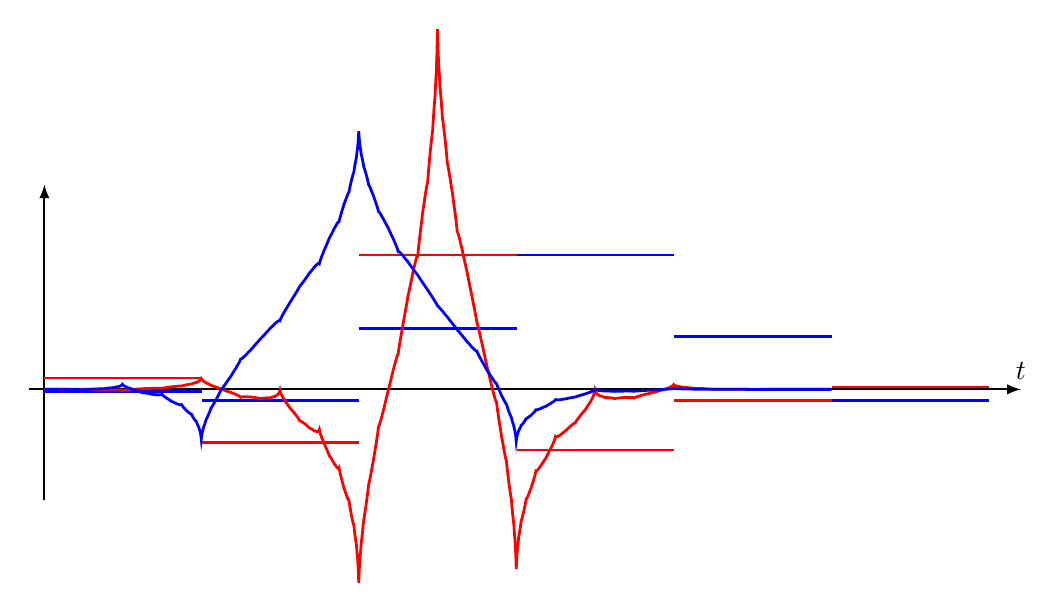
\begin{tikzpicture}[>=latex,scale=2]
\draw[->,line width=0.7pt] (-0.1,0)--(6.2,0) coordinate[label={$t$}];
\draw[->,line width=0.7pt] (0,-0.7)--(0,1.3);
\draw[color=blue,line width=1pt] (0,-0.0156557281)--(1,-0.0156557281);
\draw[color=blue,line width=1pt] (1,-0.0727326195)--(2,-0.0727326195);
\draw[color=blue,line width=1pt] (2, 0.3848648469)--(3, 0.3848648469);
\draw[color=blue,line width=1pt] (3, 0.8525720202)--(4, 0.8525720202);
\draw[color=blue,line width=1pt] (4, 0.3378976625)--(5, 0.3378976625);
\draw[color=blue,line width=1pt] (5,-0.0727326195)--(6,-0.0727326195);
\draw[color=red,line width=1pt] (0,+0.0727326195)--(1,+0.0727326195);
\draw[color=red,line width=1pt] (1,-0.3378976625)--(2,-0.3378976625);
\draw[color=red,line width=1pt] (2,+0.8525720202)--(3,+0.8525720202);
\draw[color=red,line width=1pt] (3,-0.3848648469)--(4,-0.3848648469);
\draw[color=red,line width=1pt] (4,-0.0727326195)--(5,-0.0727326195);
\draw[color=red,line width=1pt] (5,+0.0156557281)--(6,+0.0156557281);
\draw[line width=1pt,color=red] (0.00000, 0.00000)
--(0.00195, -0.00000)
--(0.00391, -0.00000)
--(0.00586, 0.00000)
--(0.00781, 0.00000)
--(0.00977, 0.00000)
--(0.01172, 0.00000)
--(0.01367, 0.00000)
--(0.01562, -0.00000)
--(0.01758, -0.00000)
--(0.01953, -0.00000)
--(0.02148, -0.00000)
--(0.02344, -0.00000)
--(0.02539, -0.00000)
--(0.02734, -0.00000)
--(0.02930, -0.00000)
--(0.03125, -0.00000)
--(0.03320, 0.00000)
--(0.03516, 0.00000)
--(0.03711, 0.00000)
--(0.03906, 0.00000)
--(0.04102, 0.00000)
--(0.04297, 0.00000)
--(0.04492, 0.00000)
--(0.04688, 0.00000)
--(0.04883, 0.00000)
--(0.05078, 0.00000)
--(0.05273, 0.00000)
--(0.05469, 0.00000)
--(0.05664, 0.00001)
--(0.05859, 0.00001)
--(0.06055, 0.00000)
--(0.06250, 0.00000)
--(0.06445, 0.00000)
--(0.06641, 0.00000)
--(0.06836, -0.00000)
--(0.07031, -0.00000)
--(0.07227, -0.00000)
--(0.07422, -0.00000)
--(0.07617, -0.00001)
--(0.07812, -0.00001)
--(0.08008, -0.00001)
--(0.08203, -0.00001)
--(0.08398, -0.00001)
--(0.08594, -0.00001)
--(0.08789, -0.00001)
--(0.08984, -0.00001)
--(0.09180, -0.00001)
--(0.09375, -0.00001)
--(0.09570, -0.00002)
--(0.09766, -0.00002)
--(0.09961, -0.00002)
--(0.10156, -0.00002)
--(0.10352, -0.00002)
--(0.10547, -0.00002)
--(0.10742, -0.00003)
--(0.10938, -0.00003)
--(0.11133, -0.00003)
--(0.11328, -0.00004)
--(0.11523, -0.00004)
--(0.11719, -0.00005)
--(0.11914, -0.00006)
--(0.12109, -0.00007)
--(0.12305, -0.00006)
--(0.12500, -0.00005)
--(0.12695, -0.00004)
--(0.12891, -0.00003)
--(0.13086, -0.00002)
--(0.13281, -0.00002)
--(0.13477, -0.00001)
--(0.13672, -0.00000)
--(0.13867, 0.00000)
--(0.14062, 0.00001)
--(0.14258, 0.00001)
--(0.14453, 0.00002)
--(0.14648, 0.00003)
--(0.14844, 0.00003)
--(0.15039, 0.00004)
--(0.15234, 0.00005)
--(0.15430, 0.00005)
--(0.15625, 0.00005)
--(0.15820, 0.00005)
--(0.16016, 0.00006)
--(0.16211, 0.00006)
--(0.16406, 0.00006)
--(0.16602, 0.00007)
--(0.16797, 0.00007)
--(0.16992, 0.00007)
--(0.17188, 0.00007)
--(0.17383, 0.00008)
--(0.17578, 0.00008)
--(0.17773, 0.00008)
--(0.17969, 0.00008)
--(0.18164, 0.00008)
--(0.18359, 0.00007)
--(0.18555, 0.00009)
--(0.18750, 0.00010)
--(0.18945, 0.00012)
--(0.19141, 0.00013)
--(0.19336, 0.00014)
--(0.19531, 0.00015)
--(0.19727, 0.00016)
--(0.19922, 0.00018)
--(0.20117, 0.00018)
--(0.20312, 0.00019)
--(0.20508, 0.00020)
--(0.20703, 0.00021)
--(0.20898, 0.00021)
--(0.21094, 0.00022)
--(0.21289, 0.00022)
--(0.21484, 0.00022)
--(0.21680, 0.00025)
--(0.21875, 0.00027)
--(0.22070, 0.00029)
--(0.22266, 0.00031)
--(0.22461, 0.00032)
--(0.22656, 0.00034)
--(0.22852, 0.00035)
--(0.23047, 0.00036)
--(0.23242, 0.00039)
--(0.23438, 0.00042)
--(0.23633, 0.00045)
--(0.23828, 0.00047)
--(0.24023, 0.00051)
--(0.24219, 0.00055)
--(0.24414, 0.00061)
--(0.24609, 0.00069)
--(0.24805, 0.00061)
--(0.25000, 0.00054)
--(0.25195, 0.00049)
--(0.25391, 0.00044)
--(0.25586, 0.00040)
--(0.25781, 0.00036)
--(0.25977, 0.00032)
--(0.26172, 0.00027)
--(0.26367, 0.00024)
--(0.26562, 0.00021)
--(0.26758, 0.00018)
--(0.26953, 0.00015)
--(0.27148, 0.00012)
--(0.27344, 0.00008)
--(0.27539, 0.00005)
--(0.27734, 0.00001)
--(0.27930, -0.00001)
--(0.28125, -0.00004)
--(0.28320, -0.00006)
--(0.28516, -0.00009)
--(0.28711, -0.00012)
--(0.28906, -0.00014)
--(0.29102, -0.00017)
--(0.29297, -0.00019)
--(0.29492, -0.00022)
--(0.29688, -0.00026)
--(0.29883, -0.00029)
--(0.30078, -0.00031)
--(0.30273, -0.00035)
--(0.30469, -0.00038)
--(0.30664, -0.00042)
--(0.30859, -0.00046)
--(0.31055, -0.00047)
--(0.31250, -0.00047)
--(0.31445, -0.00048)
--(0.31641, -0.00049)
--(0.31836, -0.00051)
--(0.32031, -0.00052)
--(0.32227, -0.00053)
--(0.32422, -0.00054)
--(0.32617, -0.00056)
--(0.32812, -0.00058)
--(0.33008, -0.00060)
--(0.33203, -0.00061)
--(0.33398, -0.00063)
--(0.33594, -0.00065)
--(0.33789, -0.00067)
--(0.33984, -0.00069)
--(0.34180, -0.00070)
--(0.34375, -0.00070)
--(0.34570, -0.00071)
--(0.34766, -0.00072)
--(0.34961, -0.00073)
--(0.35156, -0.00074)
--(0.35352, -0.00076)
--(0.35547, -0.00077)
--(0.35742, -0.00077)
--(0.35938, -0.00077)
--(0.36133, -0.00077)
--(0.36328, -0.00078)
--(0.36523, -0.00076)
--(0.36719, -0.00076)
--(0.36914, -0.00073)
--(0.37109, -0.00068)
--(0.37305, -0.00078)
--(0.37500, -0.00086)
--(0.37695, -0.00093)
--(0.37891, -0.00100)
--(0.38086, -0.00106)
--(0.38281, -0.00112)
--(0.38477, -0.00118)
--(0.38672, -0.00125)
--(0.38867, -0.00130)
--(0.39062, -0.00135)
--(0.39258, -0.00141)
--(0.39453, -0.00146)
--(0.39648, -0.00152)
--(0.39844, -0.00158)
--(0.40039, -0.00164)
--(0.40234, -0.00171)
--(0.40430, -0.00174)
--(0.40625, -0.00177)
--(0.40820, -0.00181)
--(0.41016, -0.00184)
--(0.41211, -0.00188)
--(0.41406, -0.00192)
--(0.41602, -0.00197)
--(0.41797, -0.00201)
--(0.41992, -0.00204)
--(0.42188, -0.00207)
--(0.42383, -0.00210)
--(0.42578, -0.00214)
--(0.42773, -0.00216)
--(0.42969, -0.00218)
--(0.43164, -0.00218)
--(0.43359, -0.00216)
--(0.43555, -0.00229)
--(0.43750, -0.00241)
--(0.43945, -0.00251)
--(0.44141, -0.00261)
--(0.44336, -0.00270)
--(0.44531, -0.00279)
--(0.44727, -0.00289)
--(0.44922, -0.00300)
--(0.45117, -0.00306)
--(0.45312, -0.00313)
--(0.45508, -0.00321)
--(0.45703, -0.00328)
--(0.45898, -0.00334)
--(0.46094, -0.00341)
--(0.46289, -0.00345)
--(0.46484, -0.00348)
--(0.46680, -0.00365)
--(0.46875, -0.00380)
--(0.47070, -0.00395)
--(0.47266, -0.00410)
--(0.47461, -0.00422)
--(0.47656, -0.00434)
--(0.47852, -0.00444)
--(0.48047, -0.00453)
--(0.48242, -0.00475)
--(0.48438, -0.00497)
--(0.48633, -0.00516)
--(0.48828, -0.00532)
--(0.49023, -0.00563)
--(0.49219, -0.00590)
--(0.49414, -0.00632)
--(0.49609, -0.00689)
--(0.49805, -0.00637)
--(0.50000, -0.00593)
--(0.50195, -0.00560)
--(0.50391, -0.00526)
--(0.50586, -0.00502)
--(0.50781, -0.00478)
--(0.50977, -0.00451)
--(0.51172, -0.00422)
--(0.51367, -0.00405)
--(0.51562, -0.00387)
--(0.51758, -0.00368)
--(0.51953, -0.00350)
--(0.52148, -0.00328)
--(0.52344, -0.00307)
--(0.52539, -0.00285)
--(0.52734, -0.00261)
--(0.52930, -0.00249)
--(0.53125, -0.00235)
--(0.53320, -0.00221)
--(0.53516, -0.00207)
--(0.53711, -0.00192)
--(0.53906, -0.00176)
--(0.54102, -0.00162)
--(0.54297, -0.00147)
--(0.54492, -0.00130)
--(0.54688, -0.00114)
--(0.54883, -0.00097)
--(0.55078, -0.00081)
--(0.55273, -0.00064)
--(0.55469, -0.00047)
--(0.55664, -0.00029)
--(0.55859, -0.00010)
--(0.56055, 0.00001)
--(0.56250, 0.00012)
--(0.56445, 0.00024)
--(0.56641, 0.00036)
--(0.56836, 0.00049)
--(0.57031, 0.00061)
--(0.57227, 0.00074)
--(0.57422, 0.00086)
--(0.57617, 0.00099)
--(0.57812, 0.00112)
--(0.58008, 0.00125)
--(0.58203, 0.00138)
--(0.58398, 0.00151)
--(0.58594, 0.00163)
--(0.58789, 0.00175)
--(0.58984, 0.00186)
--(0.59180, 0.00202)
--(0.59375, 0.00218)
--(0.59570, 0.00233)
--(0.59766, 0.00248)
--(0.59961, 0.00263)
--(0.60156, 0.00277)
--(0.60352, 0.00291)
--(0.60547, 0.00305)
--(0.60742, 0.00322)
--(0.60938, 0.00339)
--(0.61133, 0.00355)
--(0.61328, 0.00370)
--(0.61523, 0.00390)
--(0.61719, 0.00408)
--(0.61914, 0.00430)
--(0.62109, 0.00455)
--(0.62305, 0.00454)
--(0.62500, 0.00454)
--(0.62695, 0.00457)
--(0.62891, 0.00460)
--(0.63086, 0.00466)
--(0.63281, 0.00471)
--(0.63477, 0.00476)
--(0.63672, 0.00480)
--(0.63867, 0.00487)
--(0.64062, 0.00494)
--(0.64258, 0.00500)
--(0.64453, 0.00507)
--(0.64648, 0.00513)
--(0.64844, 0.00518)
--(0.65039, 0.00524)
--(0.65234, 0.00528)
--(0.65430, 0.00538)
--(0.65625, 0.00547)
--(0.65820, 0.00556)
--(0.66016, 0.00564)
--(0.66211, 0.00572)
--(0.66406, 0.00581)
--(0.66602, 0.00589)
--(0.66797, 0.00597)
--(0.66992, 0.00606)
--(0.67188, 0.00615)
--(0.67383, 0.00623)
--(0.67578, 0.00632)
--(0.67773, 0.00642)
--(0.67969, 0.00651)
--(0.68164, 0.00662)
--(0.68359, 0.00675)
--(0.68555, 0.00676)
--(0.68750, 0.00679)
--(0.68945, 0.00682)
--(0.69141, 0.00685)
--(0.69336, 0.00689)
--(0.69531, 0.00693)
--(0.69727, 0.00697)
--(0.69922, 0.00700)
--(0.70117, 0.00706)
--(0.70312, 0.00712)
--(0.70508, 0.00718)
--(0.70703, 0.00723)
--(0.70898, 0.00730)
--(0.71094, 0.00736)
--(0.71289, 0.00745)
--(0.71484, 0.00755)
--(0.71680, 0.00752)
--(0.71875, 0.00750)
--(0.72070, 0.00749)
--(0.72266, 0.00747)
--(0.72461, 0.00749)
--(0.72656, 0.00751)
--(0.72852, 0.00754)
--(0.73047, 0.00759)
--(0.73242, 0.00751)
--(0.73438, 0.00743)
--(0.73633, 0.00739)
--(0.73828, 0.00737)
--(0.74023, 0.00722)
--(0.74219, 0.00710)
--(0.74414, 0.00685)
--(0.74609, 0.00647)
--(0.74805, 0.00705)
--(0.75000, 0.00756)
--(0.75195, 0.00796)
--(0.75391, 0.00839)
--(0.75586, 0.00872)
--(0.75781, 0.00905)
--(0.75977, 0.00941)
--(0.76172, 0.00978)
--(0.76367, 0.01005)
--(0.76562, 0.01033)
--(0.76758, 0.01062)
--(0.76953, 0.01090)
--(0.77148, 0.01121)
--(0.77344, 0.01151)
--(0.77539, 0.01182)
--(0.77734, 0.01214)
--(0.77930, 0.01238)
--(0.78125, 0.01263)
--(0.78320, 0.01289)
--(0.78516, 0.01315)
--(0.78711, 0.01341)
--(0.78906, 0.01367)
--(0.79102, 0.01393)
--(0.79297, 0.01418)
--(0.79492, 0.01447)
--(0.79688, 0.01476)
--(0.79883, 0.01504)
--(0.80078, 0.01532)
--(0.80273, 0.01563)
--(0.80469, 0.01593)
--(0.80664, 0.01627)
--(0.80859, 0.01664)
--(0.81055, 0.01676)
--(0.81250, 0.01689)
--(0.81445, 0.01705)
--(0.81641, 0.01720)
--(0.81836, 0.01738)
--(0.82031, 0.01756)
--(0.82227, 0.01773)
--(0.82422, 0.01789)
--(0.82617, 0.01810)
--(0.82812, 0.01831)
--(0.83008, 0.01851)
--(0.83203, 0.01870)
--(0.83398, 0.01891)
--(0.83594, 0.01912)
--(0.83789, 0.01934)
--(0.83984, 0.01958)
--(0.84180, 0.01970)
--(0.84375, 0.01984)
--(0.84570, 0.01998)
--(0.84766, 0.02011)
--(0.84961, 0.02028)
--(0.85156, 0.02044)
--(0.85352, 0.02062)
--(0.85547, 0.02082)
--(0.85742, 0.02088)
--(0.85938, 0.02096)
--(0.86133, 0.02106)
--(0.86328, 0.02119)
--(0.86523, 0.02118)
--(0.86719, 0.02121)
--(0.86914, 0.02110)
--(0.87109, 0.02087)
--(0.87305, 0.02160)
--(0.87500, 0.02226)
--(0.87695, 0.02282)
--(0.87891, 0.02340)
--(0.88086, 0.02388)
--(0.88281, 0.02436)
--(0.88477, 0.02487)
--(0.88672, 0.02539)
--(0.88867, 0.02582)
--(0.89062, 0.02627)
--(0.89258, 0.02672)
--(0.89453, 0.02716)
--(0.89648, 0.02765)
--(0.89844, 0.02812)
--(0.90039, 0.02863)
--(0.90234, 0.02918)
--(0.90430, 0.02947)
--(0.90625, 0.02977)
--(0.90820, 0.03011)
--(0.91016, 0.03043)
--(0.91211, 0.03080)
--(0.91406, 0.03116)
--(0.91602, 0.03154)
--(0.91797, 0.03193)
--(0.91992, 0.03221)
--(0.92188, 0.03249)
--(0.92383, 0.03280)
--(0.92578, 0.03314)
--(0.92773, 0.03334)
--(0.92969, 0.03357)
--(0.93164, 0.03367)
--(0.93359, 0.03364)
--(0.93555, 0.03458)
--(0.93750, 0.03545)
--(0.93945, 0.03622)
--(0.94141, 0.03700)
--(0.94336, 0.03770)
--(0.94531, 0.03840)
--(0.94727, 0.03916)
--(0.94922, 0.03994)
--(0.95117, 0.04047)
--(0.95312, 0.04101)
--(0.95508, 0.04160)
--(0.95703, 0.04220)
--(0.95898, 0.04269)
--(0.96094, 0.04321)
--(0.96289, 0.04359)
--(0.96484, 0.04385)
--(0.96680, 0.04507)
--(0.96875, 0.04622)
--(0.97070, 0.04729)
--(0.97266, 0.04840)
--(0.97461, 0.04925)
--(0.97656, 0.05015)
--(0.97852, 0.05093)
--(0.98047, 0.05157)
--(0.98242, 0.05318)
--(0.98438, 0.05475)
--(0.98633, 0.05605)
--(0.98828, 0.05723)
--(0.99023, 0.05938)
--(0.99219, 0.06129)
--(0.99414, 0.06418)
--(0.99609, 0.06806)
--(0.99805, 0.06468)
--(1.00000, 0.06183)
--(1.00195, 0.05976)
--(1.00391, 0.05752)
--(1.00586, 0.05604)
--(1.00781, 0.05451)
--(1.00977, 0.05280)
--(1.01172, 0.05099)
--(1.01367, 0.04993)
--(1.01562, 0.04882)
--(1.01758, 0.04764)
--(1.01953, 0.04649)
--(1.02148, 0.04516)
--(1.02344, 0.04385)
--(1.02539, 0.04246)
--(1.02734, 0.04097)
--(1.02930, 0.04021)
--(1.03125, 0.03941)
--(1.03320, 0.03852)
--(1.03516, 0.03765)
--(1.03711, 0.03671)
--(1.03906, 0.03578)
--(1.04102, 0.03488)
--(1.04297, 0.03400)
--(1.04492, 0.03294)
--(1.04688, 0.03188)
--(1.04883, 0.03087)
--(1.05078, 0.02986)
--(1.05273, 0.02876)
--(1.05469, 0.02768)
--(1.05664, 0.02650)
--(1.05859, 0.02520)
--(1.06055, 0.02471)
--(1.06250, 0.02416)
--(1.06445, 0.02352)
--(1.06641, 0.02290)
--(1.06836, 0.02220)
--(1.07031, 0.02150)
--(1.07227, 0.02083)
--(1.07422, 0.02016)
--(1.07617, 0.01941)
--(1.07812, 0.01868)
--(1.08008, 0.01794)
--(1.08203, 0.01720)
--(1.08398, 0.01649)
--(1.08594, 0.01578)
--(1.08789, 0.01508)
--(1.08984, 0.01440)
--(1.09180, 0.01359)
--(1.09375, 0.01278)
--(1.09570, 0.01199)
--(1.09766, 0.01119)
--(1.09961, 0.01042)
--(1.10156, 0.00965)
--(1.10352, 0.00887)
--(1.10547, 0.00811)
--(1.10742, 0.00730)
--(1.10938, 0.00649)
--(1.11133, 0.00570)
--(1.11328, 0.00491)
--(1.11523, 0.00407)
--(1.11719, 0.00324)
--(1.11914, 0.00236)
--(1.12109, 0.00143)
--(1.12305, 0.00088)
--(1.12500, 0.00031)
--(1.12695, -0.00030)
--(1.12891, -0.00091)
--(1.13086, -0.00155)
--(1.13281, -0.00219)
--(1.13477, -0.00282)
--(1.13672, -0.00345)
--(1.13867, -0.00412)
--(1.14062, -0.00479)
--(1.14258, -0.00546)
--(1.14453, -0.00612)
--(1.14648, -0.00679)
--(1.14844, -0.00745)
--(1.15039, -0.00812)
--(1.15234, -0.00879)
--(1.15430, -0.00944)
--(1.15625, -0.01008)
--(1.15820, -0.01073)
--(1.16016, -0.01138)
--(1.16211, -0.01204)
--(1.16406, -0.01269)
--(1.16602, -0.01336)
--(1.16797, -0.01404)
--(1.16992, -0.01464)
--(1.17188, -0.01525)
--(1.17383, -0.01588)
--(1.17578, -0.01651)
--(1.17773, -0.01708)
--(1.17969, -0.01767)
--(1.18164, -0.01819)
--(1.18359, -0.01863)
--(1.18555, -0.01959)
--(1.18750, -0.02050)
--(1.18945, -0.02136)
--(1.19141, -0.02223)
--(1.19336, -0.02306)
--(1.19531, -0.02388)
--(1.19727, -0.02473)
--(1.19922, -0.02560)
--(1.20117, -0.02634)
--(1.20312, -0.02710)
--(1.20508, -0.02787)
--(1.20703, -0.02865)
--(1.20898, -0.02938)
--(1.21094, -0.03013)
--(1.21289, -0.03082)
--(1.21484, -0.03145)
--(1.21680, -0.03249)
--(1.21875, -0.03351)
--(1.22070, -0.03449)
--(1.22266, -0.03549)
--(1.22461, -0.03637)
--(1.22656, -0.03728)
--(1.22852, -0.03813)
--(1.23047, -0.03892)
--(1.23242, -0.04014)
--(1.23438, -0.04134)
--(1.23633, -0.04242)
--(1.23828, -0.04345)
--(1.24023, -0.04490)
--(1.24219, -0.04625)
--(1.24414, -0.04802)
--(1.24609, -0.05023)
--(1.24805, -0.04927)
--(1.25000, -0.04855)
--(1.25195, -0.04816)
--(1.25391, -0.04770)
--(1.25586, -0.04757)
--(1.25781, -0.04742)
--(1.25977, -0.04719)
--(1.26172, -0.04692)
--(1.26367, -0.04698)
--(1.26562, -0.04701)
--(1.26758, -0.04702)
--(1.26953, -0.04703)
--(1.27148, -0.04698)
--(1.27344, -0.04693)
--(1.27539, -0.04685)
--(1.27734, -0.04674)
--(1.27930, -0.04690)
--(1.28125, -0.04704)
--(1.28320, -0.04715)
--(1.28516, -0.04726)
--(1.28711, -0.04736)
--(1.28906, -0.04745)
--(1.29102, -0.04757)
--(1.29297, -0.04770)
--(1.29492, -0.04771)
--(1.29688, -0.04773)
--(1.29883, -0.04777)
--(1.30078, -0.04782)
--(1.30273, -0.04779)
--(1.30469, -0.04778)
--(1.30664, -0.04768)
--(1.30859, -0.04749)
--(1.31055, -0.04797)
--(1.31250, -0.04839)
--(1.31445, -0.04875)
--(1.31641, -0.04912)
--(1.31836, -0.04942)
--(1.32031, -0.04973)
--(1.32227, -0.05006)
--(1.32422, -0.05041)
--(1.32617, -0.05065)
--(1.32812, -0.05089)
--(1.33008, -0.05115)
--(1.33203, -0.05141)
--(1.33398, -0.05165)
--(1.33594, -0.05189)
--(1.33789, -0.05211)
--(1.33984, -0.05229)
--(1.34180, -0.05270)
--(1.34375, -0.05308)
--(1.34570, -0.05346)
--(1.34766, -0.05384)
--(1.34961, -0.05415)
--(1.35156, -0.05448)
--(1.35352, -0.05478)
--(1.35547, -0.05503)
--(1.35742, -0.05555)
--(1.35938, -0.05606)
--(1.36133, -0.05650)
--(1.36328, -0.05691)
--(1.36523, -0.05757)
--(1.36719, -0.05817)
--(1.36914, -0.05903)
--(1.37109, -0.06016)
--(1.37305, -0.05934)
--(1.37500, -0.05867)
--(1.37695, -0.05821)
--(1.37891, -0.05770)
--(1.38086, -0.05740)
--(1.38281, -0.05708)
--(1.38477, -0.05673)
--(1.38672, -0.05635)
--(1.38867, -0.05613)
--(1.39062, -0.05589)
--(1.39258, -0.05564)
--(1.39453, -0.05542)
--(1.39648, -0.05509)
--(1.39844, -0.05479)
--(1.40039, -0.05442)
--(1.40234, -0.05397)
--(1.40430, -0.05406)
--(1.40625, -0.05411)
--(1.40820, -0.05411)
--(1.41016, -0.05413)
--(1.41211, -0.05404)
--(1.41406, -0.05397)
--(1.41602, -0.05388)
--(1.41797, -0.05374)
--(1.41992, -0.05386)
--(1.42188, -0.05397)
--(1.42383, -0.05400)
--(1.42578, -0.05400)
--(1.42773, -0.05428)
--(1.42969, -0.05449)
--(1.43164, -0.05497)
--(1.43359, -0.05574)
--(1.43555, -0.05444)
--(1.43750, -0.05330)
--(1.43945, -0.05239)
--(1.44141, -0.05144)
--(1.44336, -0.05065)
--(1.44531, -0.04985)
--(1.44727, -0.04897)
--(1.44922, -0.04800)
--(1.45117, -0.04759)
--(1.45312, -0.04714)
--(1.45508, -0.04659)
--(1.45703, -0.04601)
--(1.45898, -0.04568)
--(1.46094, -0.04528)
--(1.46289, -0.04516)
--(1.46484, -0.04533)
--(1.46680, -0.04344)
--(1.46875, -0.04171)
--(1.47070, -0.04015)
--(1.47266, -0.03850)
--(1.47461, -0.03739)
--(1.47656, -0.03620)
--(1.47852, -0.03526)
--(1.48047, -0.03460)
--(1.48242, -0.03189)
--(1.48438, -0.02928)
--(1.48633, -0.02722)
--(1.48828, -0.02544)
--(1.49023, -0.02160)
--(1.49219, -0.01825)
--(1.49414, -0.01285)
--(1.49609, -0.00534)
--(1.49805, -0.01319)
--(1.50000, -0.01989)
--(1.50195, -0.02497)
--(1.50391, -0.03038)
--(1.50586, -0.03421)
--(1.50781, -0.03813)
--(1.50977, -0.04244)
--(1.51172, -0.04696)
--(1.51367, -0.04989)
--(1.51562, -0.05295)
--(1.51758, -0.05614)
--(1.51953, -0.05927)
--(1.52148, -0.06279)
--(1.52344, -0.06624)
--(1.52539, -0.06990)
--(1.52734, -0.07378)
--(1.52930, -0.07603)
--(1.53125, -0.07839)
--(1.53320, -0.08093)
--(1.53516, -0.08344)
--(1.53711, -0.08609)
--(1.53906, -0.08874)
--(1.54102, -0.09133)
--(1.54297, -0.09387)
--(1.54492, -0.09675)
--(1.54688, -0.09961)
--(1.54883, -0.10240)
--(1.55078, -0.10518)
--(1.55273, -0.10811)
--(1.55469, -0.11100)
--(1.55664, -0.11405)
--(1.55859, -0.11727)
--(1.56055, -0.11927)
--(1.56250, -0.12135)
--(1.56445, -0.12356)
--(1.56641, -0.12575)
--(1.56836, -0.12807)
--(1.57031, -0.13038)
--(1.57227, -0.13267)
--(1.57422, -0.13496)
--(1.57617, -0.13729)
--(1.57812, -0.13962)
--(1.58008, -0.14196)
--(1.58203, -0.14431)
--(1.58398, -0.14655)
--(1.58594, -0.14882)
--(1.58789, -0.15100)
--(1.58984, -0.15308)
--(1.59180, -0.15586)
--(1.59375, -0.15859)
--(1.59570, -0.16125)
--(1.59766, -0.16395)
--(1.59961, -0.16648)
--(1.60156, -0.16904)
--(1.60352, -0.17153)
--(1.60547, -0.17396)
--(1.60742, -0.17690)
--(1.60938, -0.17981)
--(1.61133, -0.18259)
--(1.61328, -0.18529)
--(1.61523, -0.18853)
--(1.61719, -0.19164)
--(1.61914, -0.19528)
--(1.62109, -0.19947)
--(1.62305, -0.19968)
--(1.62500, -0.20018)
--(1.62695, -0.20111)
--(1.62891, -0.20195)
--(1.63086, -0.20320)
--(1.63281, -0.20444)
--(1.63477, -0.20557)
--(1.63672, -0.20666)
--(1.63867, -0.20811)
--(1.64062, -0.20953)
--(1.64258, -0.21093)
--(1.64453, -0.21236)
--(1.64648, -0.21363)
--(1.64844, -0.21494)
--(1.65039, -0.21615)
--(1.65234, -0.21726)
--(1.65430, -0.21911)
--(1.65625, -0.22090)
--(1.65820, -0.22261)
--(1.66016, -0.22435)
--(1.66211, -0.22598)
--(1.66406, -0.22761)
--(1.66602, -0.22924)
--(1.66797, -0.23083)
--(1.66992, -0.23261)
--(1.67188, -0.23438)
--(1.67383, -0.23609)
--(1.67578, -0.23777)
--(1.67773, -0.23969)
--(1.67969, -0.24155)
--(1.68164, -0.24364)
--(1.68359, -0.24596)
--(1.68555, -0.24657)
--(1.68750, -0.24730)
--(1.68945, -0.24823)
--(1.69141, -0.24912)
--(1.69336, -0.25014)
--(1.69531, -0.25116)
--(1.69727, -0.25210)
--(1.69922, -0.25297)
--(1.70117, -0.25433)
--(1.70312, -0.25567)
--(1.70508, -0.25691)
--(1.70703, -0.25812)
--(1.70898, -0.25956)
--(1.71094, -0.26095)
--(1.71289, -0.26259)
--(1.71484, -0.26451)
--(1.71680, -0.26448)
--(1.71875, -0.26461)
--(1.72070, -0.26489)
--(1.72266, -0.26509)
--(1.72461, -0.26581)
--(1.72656, -0.26644)
--(1.72852, -0.26730)
--(1.73047, -0.26843)
--(1.73242, -0.26764)
--(1.73438, -0.26695)
--(1.73633, -0.26677)
--(1.73828, -0.26685)
--(1.74023, -0.26500)
--(1.74219, -0.26361)
--(1.74414, -0.26031)
--(1.74609, -0.25503)
--(1.74805, -0.26412)
--(1.75000, -0.27214)
--(1.75195, -0.27864)
--(1.75391, -0.28545)
--(1.75586, -0.29079)
--(1.75781, -0.29621)
--(1.75977, -0.30201)
--(1.76172, -0.30800)
--(1.76367, -0.31246)
--(1.76562, -0.31703)
--(1.76758, -0.32175)
--(1.76953, -0.32641)
--(1.77148, -0.33138)
--(1.77344, -0.33631)
--(1.77539, -0.34137)
--(1.77734, -0.34659)
--(1.77930, -0.35067)
--(1.78125, -0.35484)
--(1.78320, -0.35914)
--(1.78516, -0.36343)
--(1.78711, -0.36776)
--(1.78906, -0.37209)
--(1.79102, -0.37632)
--(1.79297, -0.38046)
--(1.79492, -0.38528)
--(1.79688, -0.39006)
--(1.79883, -0.39468)
--(1.80078, -0.39924)
--(1.80273, -0.40430)
--(1.80469, -0.40924)
--(1.80664, -0.41470)
--(1.80859, -0.42069)
--(1.81055, -0.42280)
--(1.81250, -0.42521)
--(1.81445, -0.42803)
--(1.81641, -0.43077)
--(1.81836, -0.43386)
--(1.82031, -0.43695)
--(1.82227, -0.43989)
--(1.82422, -0.44273)
--(1.82617, -0.44630)
--(1.82812, -0.44982)
--(1.83008, -0.45322)
--(1.83203, -0.45660)
--(1.83398, -0.46017)
--(1.83594, -0.46369)
--(1.83789, -0.46744)
--(1.83984, -0.47144)
--(1.84180, -0.47369)
--(1.84375, -0.47608)
--(1.84570, -0.47860)
--(1.84766, -0.48104)
--(1.84961, -0.48398)
--(1.85156, -0.48684)
--(1.85352, -0.48994)
--(1.85547, -0.49331)
--(1.85742, -0.49472)
--(1.85938, -0.49624)
--(1.86133, -0.49827)
--(1.86328, -0.50056)
--(1.86523, -0.50092)
--(1.86719, -0.50174)
--(1.86914, -0.50063)
--(1.87109, -0.49753)
--(1.87305, -0.50890)
--(1.87500, -0.51919)
--(1.87695, -0.52795)
--(1.87891, -0.53704)
--(1.88086, -0.54459)
--(1.88281, -0.55223)
--(1.88477, -0.56019)
--(1.88672, -0.56830)
--(1.88867, -0.57527)
--(1.89062, -0.58233)
--(1.89258, -0.58944)
--(1.89453, -0.59644)
--(1.89648, -0.60412)
--(1.89844, -0.61167)
--(1.90039, -0.61972)
--(1.90234, -0.62830)
--(1.90430, -0.63300)
--(1.90625, -0.63800)
--(1.90820, -0.64336)
--(1.91016, -0.64859)
--(1.91211, -0.65454)
--(1.91406, -0.66040)
--(1.91602, -0.66645)
--(1.91797, -0.67273)
--(1.91992, -0.67728)
--(1.92188, -0.68190)
--(1.92383, -0.68703)
--(1.92578, -0.69242)
--(1.92773, -0.69585)
--(1.92969, -0.69975)
--(1.93164, -0.70172)
--(1.93359, -0.70170)
--(1.93555, -0.71614)
--(1.93750, -0.72951)
--(1.93945, -0.74130)
--(1.94141, -0.75336)
--(1.94336, -0.76428)
--(1.94531, -0.77521)
--(1.94727, -0.78681)
--(1.94922, -0.79895)
--(1.95117, -0.80720)
--(1.95312, -0.81569)
--(1.95508, -0.82492)
--(1.95703, -0.83435)
--(1.95898, -0.84205)
--(1.96094, -0.85019)
--(1.96289, -0.85638)
--(1.96484, -0.86059)
--(1.96680, -0.87925)
--(1.96875, -0.89679)
--(1.97070, -0.91315)
--(1.97266, -0.93015)
--(1.97461, -0.94328)
--(1.97656, -0.95702)
--(1.97852, -0.96903)
--(1.98047, -0.97904)
--(1.98242, -1.00350)
--(1.98438, -1.02725)
--(1.98633, -1.04708)
--(1.98828, -1.06505)
--(1.99023, -1.09748)
--(1.99219, -1.12644)
--(1.99414, -1.16982)
--(1.99609, -1.22814)
--(1.99805, -1.17817)
--(2.00000, -1.13624)
--(2.00195, -1.10579)
--(2.00391, -1.07294)
--(2.00586, -1.05128)
--(2.00781, -1.02899)
--(2.00977, -1.00393)
--(2.01172, -0.97741)
--(2.01367, -0.96209)
--(2.01562, -0.94590)
--(2.01758, -0.92874)
--(2.01953, -0.91205)
--(2.02148, -0.89262)
--(2.02344, -0.87364)
--(2.02539, -0.85328)
--(2.02734, -0.83135)
--(2.02930, -0.82071)
--(2.03125, -0.80924)
--(2.03320, -0.79654)
--(2.03516, -0.78407)
--(2.03711, -0.77063)
--(2.03906, -0.75720)
--(2.04102, -0.74427)
--(2.04297, -0.73169)
--(2.04492, -0.71645)
--(2.04688, -0.70137)
--(2.04883, -0.68681)
--(2.05078, -0.67241)
--(2.05273, -0.65670)
--(2.05469, -0.64133)
--(2.05664, -0.62452)
--(2.05859, -0.60624)
--(2.06055, -0.59862)
--(2.06250, -0.59022)
--(2.06445, -0.58069)
--(2.06641, -0.57140)
--(2.06836, -0.56097)
--(2.07031, -0.55060)
--(2.07227, -0.54048)
--(2.07422, -0.53045)
--(2.07617, -0.51962)
--(2.07812, -0.50885)
--(2.08008, -0.49811)
--(2.08203, -0.48728)
--(2.08398, -0.47700)
--(2.08594, -0.46661)
--(2.08789, -0.45664)
--(2.08984, -0.44711)
--(2.09180, -0.43436)
--(2.09375, -0.42187)
--(2.09570, -0.40966)
--(2.09766, -0.39734)
--(2.09961, -0.38568)
--(2.10156, -0.37393)
--(2.10352, -0.36238)
--(2.10547, -0.35110)
--(2.10742, -0.33795)
--(2.10938, -0.32489)
--(2.11133, -0.31235)
--(2.11328, -0.30007)
--(2.11523, -0.28580)
--(2.11719, -0.27201)
--(2.11914, -0.25624)
--(2.12109, -0.23843)
--(2.12305, -0.23544)
--(2.12500, -0.23135)
--(2.12695, -0.22569)
--(2.12891, -0.22036)
--(2.13086, -0.21349)
--(2.13281, -0.20670)
--(2.13477, -0.20029)
--(2.13672, -0.19408)
--(2.13867, -0.18638)
--(2.14062, -0.17879)
--(2.14258, -0.17133)
--(2.14453, -0.16379)
--(2.14648, -0.15668)
--(2.14844, -0.14949)
--(2.15039, -0.14253)
--(2.15234, -0.13583)
--(2.15430, -0.12727)
--(2.15625, -0.11885)
--(2.15820, -0.11063)
--(2.16016, -0.10236)
--(2.16211, -0.09430)
--(2.16406, -0.08622)
--(2.16602, -0.07811)
--(2.16797, -0.06999)
--(2.16992, -0.06197)
--(2.17188, -0.05395)
--(2.17383, -0.04593)
--(2.17578, -0.03792)
--(2.17773, -0.02983)
--(2.17969, -0.02176)
--(2.18164, -0.01363)
--(2.18359, -0.00544)
--(2.18555, 0.00231)
--(2.18750, 0.01009)
--(2.18945, 0.01792)
--(2.19141, 0.02575)
--(2.19336, 0.03358)
--(2.19531, 0.04142)
--(2.19727, 0.04922)
--(2.19922, 0.05696)
--(2.20117, 0.06503)
--(2.20312, 0.07309)
--(2.20508, 0.08107)
--(2.20703, 0.08902)
--(2.20898, 0.09720)
--(2.21094, 0.10533)
--(2.21289, 0.11371)
--(2.21484, 0.12234)
--(2.21680, 0.12912)
--(2.21875, 0.13605)
--(2.22070, 0.14314)
--(2.22266, 0.15014)
--(2.22461, 0.15762)
--(2.22656, 0.16502)
--(2.22852, 0.17263)
--(2.23047, 0.18048)
--(2.23242, 0.18661)
--(2.23438, 0.19283)
--(2.23633, 0.19951)
--(2.23828, 0.20641)
--(2.24023, 0.21159)
--(2.24219, 0.21719)
--(2.24414, 0.22107)
--(2.24609, 0.22316)
--(2.24805, 0.23816)
--(2.25000, 0.25221)
--(2.25195, 0.26488)
--(2.25391, 0.27784)
--(2.25586, 0.28947)
--(2.25781, 0.30118)
--(2.25977, 0.31323)
--(2.26172, 0.32547)
--(2.26367, 0.33628)
--(2.26562, 0.34721)
--(2.26758, 0.35827)
--(2.26953, 0.36928)
--(2.27148, 0.38055)
--(2.27344, 0.39178)
--(2.27539, 0.40310)
--(2.27734, 0.41452)
--(2.27930, 0.42518)
--(2.28125, 0.43589)
--(2.28320, 0.44669)
--(2.28516, 0.45750)
--(2.28711, 0.46827)
--(2.28906, 0.47907)
--(2.29102, 0.48974)
--(2.29297, 0.50031)
--(2.29492, 0.51169)
--(2.29688, 0.52304)
--(2.29883, 0.53418)
--(2.30078, 0.54524)
--(2.30273, 0.55697)
--(2.30469, 0.56853)
--(2.30664, 0.58078)
--(2.30859, 0.59372)
--(2.31055, 0.60157)
--(2.31250, 0.60980)
--(2.31445, 0.61857)
--(2.31641, 0.62725)
--(2.31836, 0.63637)
--(2.32031, 0.64548)
--(2.32227, 0.65439)
--(2.32422, 0.66316)
--(2.32617, 0.67298)
--(2.32812, 0.68274)
--(2.33008, 0.69232)
--(2.33203, 0.70186)
--(2.33398, 0.71174)
--(2.33594, 0.72153)
--(2.33789, 0.73173)
--(2.33984, 0.74234)
--(2.34180, 0.74994)
--(2.34375, 0.75777)
--(2.34570, 0.76584)
--(2.34766, 0.77378)
--(2.34961, 0.78255)
--(2.35156, 0.79119)
--(2.35352, 0.80021)
--(2.35547, 0.80968)
--(2.35742, 0.81594)
--(2.35938, 0.82235)
--(2.36133, 0.82963)
--(2.36328, 0.83733)
--(2.36523, 0.84182)
--(2.36719, 0.84709)
--(2.36914, 0.84916)
--(2.37109, 0.84792)
--(2.37305, 0.87066)
--(2.37500, 0.89161)
--(2.37695, 0.91003)
--(2.37891, 0.92900)
--(2.38086, 0.94541)
--(2.38281, 0.96197)
--(2.38477, 0.97907)
--(2.38672, 0.99642)
--(2.38867, 1.01185)
--(2.39062, 1.02745)
--(2.39258, 1.04312)
--(2.39453, 1.05862)
--(2.39648, 1.07522)
--(2.39844, 1.09161)
--(2.40039, 1.10880)
--(2.40234, 1.12687)
--(2.40430, 1.13865)
--(2.40625, 1.15091)
--(2.40820, 1.16377)
--(2.41016, 1.17641)
--(2.41211, 1.19021)
--(2.41406, 1.20386)
--(2.41602, 1.21780)
--(2.41797, 1.23213)
--(2.41992, 1.24371)
--(2.42188, 1.25541)
--(2.42383, 1.26792)
--(2.42578, 1.28082)
--(2.42773, 1.29063)
--(2.42969, 1.30119)
--(2.43164, 1.30869)
--(2.43359, 1.31304)
--(2.43555, 1.34028)
--(2.43750, 1.36584)
--(2.43945, 1.38888)
--(2.44141, 1.41235)
--(2.44336, 1.43403)
--(2.44531, 1.45571)
--(2.44727, 1.47847)
--(2.44922, 1.50207)
--(2.45117, 1.51951)
--(2.45312, 1.53733)
--(2.45508, 1.55631)
--(2.45703, 1.57562)
--(2.45898, 1.59217)
--(2.46094, 1.60942)
--(2.46289, 1.62359)
--(2.46484, 1.63459)
--(2.46680, 1.66858)
--(2.46875, 1.70077)
--(2.47070, 1.73110)
--(2.47266, 1.76246)
--(2.47461, 1.78765)
--(2.47656, 1.81381)
--(2.47852, 1.83722)
--(2.48047, 1.85745)
--(2.48242, 1.90066)
--(2.48438, 1.94273)
--(2.48633, 1.97858)
--(2.48828, 2.01146)
--(2.49023, 2.06733)
--(2.49219, 2.11769)
--(2.49414, 2.19097)
--(2.49609, 2.28801)
--(2.49805, 2.21289)
--(2.50000, 2.15054)
--(2.50195, 2.10646)
--(2.50391, 2.05856)
--(2.50586, 2.02843)
--(2.50781, 1.99732)
--(2.50977, 1.96180)
--(2.51172, 1.92396)
--(2.51367, 1.90392)
--(2.51562, 1.88252)
--(2.51758, 1.85956)
--(2.51953, 1.83735)
--(2.52148, 1.81079)
--(2.52344, 1.78495)
--(2.52539, 1.75692)
--(2.52734, 1.72642)
--(2.52930, 1.71377)
--(2.53125, 1.69981)
--(2.53320, 1.68391)
--(2.53516, 1.66836)
--(2.53711, 1.65129)
--(2.53906, 1.63425)
--(2.54102, 1.61799)
--(2.54297, 1.60231)
--(2.54492, 1.58233)
--(2.54688, 1.56260)
--(2.54883, 1.54373)
--(2.55078, 1.52511)
--(2.55273, 1.50434)
--(2.55469, 1.48411)
--(2.55664, 1.46154)
--(2.55859, 1.43655)
--(2.56055, 1.42907)
--(2.56250, 1.42029)
--(2.56445, 1.40966)
--(2.56641, 1.39942)
--(2.56836, 1.38732)
--(2.57031, 1.37534)
--(2.57227, 1.36376)
--(2.57422, 1.35235)
--(2.57617, 1.33952)
--(2.57812, 1.32681)
--(2.58008, 1.31415)
--(2.58203, 1.30137)
--(2.58398, 1.28941)
--(2.58594, 1.27728)
--(2.58789, 1.26575)
--(2.58984, 1.25486)
--(2.59180, 1.23935)
--(2.59375, 1.22419)
--(2.59570, 1.20945)
--(2.59766, 1.19455)
--(2.59961, 1.18057)
--(2.60156, 1.16647)
--(2.60352, 1.15264)
--(2.60547, 1.13915)
--(2.60742, 1.12319)
--(2.60938, 1.10735)
--(2.61133, 1.09221)
--(2.61328, 1.07742)
--(2.61523, 1.05995)
--(2.61719, 1.04313)
--(2.61914, 1.02366)
--(2.62109, 1.00145)
--(2.62305, 0.99909)
--(2.62500, 0.99527)
--(2.62695, 0.98933)
--(2.62891, 0.98384)
--(2.63086, 0.97629)
--(2.63281, 0.96887)
--(2.63477, 0.96194)
--(2.63672, 0.95529)
--(2.63867, 0.94658)
--(2.64062, 0.93803)
--(2.64258, 0.92966)
--(2.64453, 0.92120)
--(2.64648, 0.91324)
--(2.64844, 0.90520)
--(2.65039, 0.89740)
--(2.65234, 0.88989)
--(2.65430, 0.88035)
--(2.65625, 0.87097)
--(2.65820, 0.86181)
--(2.66016, 0.85261)
--(2.66211, 0.84356)
--(2.66406, 0.83452)
--(2.66602, 0.82538)
--(2.66797, 0.81616)
--(2.66992, 0.80751)
--(2.67188, 0.79883)
--(2.67383, 0.79003)
--(2.67578, 0.78120)
--(2.67773, 0.77268)
--(2.67969, 0.76409)
--(2.68164, 0.75584)
--(2.68359, 0.74794)
--(2.68555, 0.73747)
--(2.68750, 0.72719)
--(2.68945, 0.71718)
--(2.69141, 0.70712)
--(2.69336, 0.69731)
--(2.69531, 0.68749)
--(2.69727, 0.67759)
--(2.69922, 0.66764)
--(2.70117, 0.65806)
--(2.70312, 0.64846)
--(2.70508, 0.63880)
--(2.70703, 0.62915)
--(2.70898, 0.61952)
--(2.71094, 0.60987)
--(2.71289, 0.60029)
--(2.71484, 0.59075)
--(2.71680, 0.58083)
--(2.71875, 0.57093)
--(2.72070, 0.56106)
--(2.72266, 0.55117)
--(2.72461, 0.54142)
--(2.72656, 0.53164)
--(2.72852, 0.52193)
--(2.73047, 0.51231)
--(2.73242, 0.50209)
--(2.73438, 0.49190)
--(2.73633, 0.48187)
--(2.73828, 0.47192)
--(2.74023, 0.46139)
--(2.74219, 0.45099)
--(2.74414, 0.44002)
--(2.74609, 0.42845)
--(2.74805, 0.42122)
--(2.75000, 0.41367)
--(2.75195, 0.40565)
--(2.75391, 0.39774)
--(2.75586, 0.38937)
--(2.75781, 0.38102)
--(2.75977, 0.37278)
--(2.76172, 0.36459)
--(2.76367, 0.35601)
--(2.76562, 0.34745)
--(2.76758, 0.33892)
--(2.76953, 0.33037)
--(2.77148, 0.32197)
--(2.77344, 0.31355)
--(2.77539, 0.30522)
--(2.77734, 0.29700)
--(2.77930, 0.28799)
--(2.78125, 0.27905)
--(2.78320, 0.27018)
--(2.78516, 0.26128)
--(2.78711, 0.25251)
--(2.78906, 0.24373)
--(2.79102, 0.23496)
--(2.79297, 0.22622)
--(2.79492, 0.21729)
--(2.79688, 0.20836)
--(2.79883, 0.19950)
--(2.80078, 0.19067)
--(2.80273, 0.18158)
--(2.80469, 0.17256)
--(2.80664, 0.16329)
--(2.80859, 0.15377)
--(2.81055, 0.14609)
--(2.81250, 0.13827)
--(2.81445, 0.13025)
--(2.81641, 0.12227)
--(2.81836, 0.11415)
--(2.82031, 0.10602)
--(2.82227, 0.09799)
--(2.82422, 0.09003)
--(2.82617, 0.08153)
--(2.82812, 0.07307)
--(2.83008, 0.06471)
--(2.83203, 0.05638)
--(2.83398, 0.04778)
--(2.83594, 0.03926)
--(2.83789, 0.03044)
--(2.83984, 0.02132)
--(2.84180, 0.01437)
--(2.84375, 0.00725)
--(2.84570, -0.00004)
--(2.84766, -0.00724)
--(2.84961, -0.01502)
--(2.85156, -0.02270)
--(2.85352, -0.03064)
--(2.85547, -0.03888)
--(2.85742, -0.04498)
--(2.85938, -0.05119)
--(2.86133, -0.05797)
--(2.86328, -0.06503)
--(2.86523, -0.06996)
--(2.86719, -0.07539)
--(2.86914, -0.07870)
--(2.87109, -0.07980)
--(2.87305, -0.09690)
--(2.87500, -0.11281)
--(2.87695, -0.12703)
--(2.87891, -0.14161)
--(2.88086, -0.15449)
--(2.88281, -0.16747)
--(2.88477, -0.18082)
--(2.88672, -0.19433)
--(2.88867, -0.20654)
--(2.89062, -0.21886)
--(2.89258, -0.23123)
--(2.89453, -0.24349)
--(2.89648, -0.25647)
--(2.89844, -0.26931)
--(2.90039, -0.28266)
--(2.90234, -0.29657)
--(2.90430, -0.30647)
--(2.90625, -0.31667)
--(2.90820, -0.32725)
--(2.91016, -0.33770)
--(2.91211, -0.34888)
--(2.91406, -0.35997)
--(2.91602, -0.37123)
--(2.91797, -0.38272)
--(2.91992, -0.39254)
--(2.92188, -0.40244)
--(2.92383, -0.41283)
--(2.92578, -0.42346)
--(2.92773, -0.43220)
--(2.92969, -0.44140)
--(2.93164, -0.44872)
--(2.93359, -0.45411)
--(2.93555, -0.47353)
--(2.93750, -0.49191)
--(2.93945, -0.50876)
--(2.94141, -0.52586)
--(2.94336, -0.54187)
--(2.94531, -0.55789)
--(2.94727, -0.57456)
--(2.94922, -0.59176)
--(2.95117, -0.60515)
--(2.95312, -0.61879)
--(2.95508, -0.63314)
--(2.95703, -0.64769)
--(2.95898, -0.66054)
--(2.96094, -0.67382)
--(2.96289, -0.68519)
--(2.96484, -0.69461)
--(2.96680, -0.71823)
--(2.96875, -0.74075)
--(2.97070, -0.76211)
--(2.97266, -0.78411)
--(2.97461, -0.80229)
--(2.97656, -0.82108)
--(2.97852, -0.83817)
--(2.98047, -0.85329)
--(2.98242, -0.88261)
--(2.98438, -0.91122)
--(2.98633, -0.93599)
--(2.98828, -0.95893)
--(2.99023, -0.99606)
--(2.99219, -1.02979)
--(2.99414, -1.07767)
--(2.99609, -1.14023)
--(2.99805, -1.09647)
--(3.00000, -1.06060)
--(3.00195, -1.03601)
--(3.00391, -1.00906)
--(3.00586, -0.99309)
--(3.00781, -0.97650)
--(3.00977, -0.95720)
--(3.01172, -0.93646)
--(3.01367, -0.92672)
--(3.01562, -0.91614)
--(3.01758, -0.90460)
--(3.01953, -0.89351)
--(3.02148, -0.87974)
--(3.02344, -0.86642)
--(3.02539, -0.85175)
--(3.02734, -0.83555)
--(3.02930, -0.83036)
--(3.03125, -0.82436)
--(3.03320, -0.81716)
--(3.03516, -0.81017)
--(3.03711, -0.80226)
--(3.03906, -0.79436)
--(3.04102, -0.78695)
--(3.04297, -0.77990)
--(3.04492, -0.77017)
--(3.04688, -0.76059)
--(3.04883, -0.75155)
--(3.05078, -0.74268)
--(3.05273, -0.73245)
--(3.05469, -0.72256)
--(3.05664, -0.71120)
--(3.05859, -0.69833)
--(3.06055, -0.69643)
--(3.06250, -0.69371)
--(3.06445, -0.68983)
--(3.06641, -0.68620)
--(3.06836, -0.68141)
--(3.07031, -0.67669)
--(3.07227, -0.67222)
--(3.07422, -0.66787)
--(3.07617, -0.66260)
--(3.07812, -0.65740)
--(3.08008, -0.65225)
--(3.08203, -0.64702)
--(3.08398, -0.64228)
--(3.08594, -0.63744)
--(3.08789, -0.63295)
--(3.08984, -0.62884)
--(3.09180, -0.62201)
--(3.09375, -0.61539)
--(3.09570, -0.60902)
--(3.09766, -0.60255)
--(3.09961, -0.59662)
--(3.10156, -0.59061)
--(3.10352, -0.58476)
--(3.10547, -0.57910)
--(3.10742, -0.57205)
--(3.10938, -0.56507)
--(3.11133, -0.55848)
--(3.11328, -0.55209)
--(3.11523, -0.54419)
--(3.11719, -0.53665)
--(3.11914, -0.52761)
--(3.12109, -0.51703)
--(3.12305, -0.51767)
--(3.12500, -0.51747)
--(3.12695, -0.51609)
--(3.12891, -0.51495)
--(3.13086, -0.51266)
--(3.13281, -0.51043)
--(3.13477, -0.50849)
--(3.13672, -0.50671)
--(3.13867, -0.50374)
--(3.14062, -0.50086)
--(3.14258, -0.49809)
--(3.14453, -0.49527)
--(3.14648, -0.49271)
--(3.14844, -0.49011)
--(3.15039, -0.48763)
--(3.15234, -0.48529)
--(3.15430, -0.48197)
--(3.15625, -0.47871)
--(3.15820, -0.47557)
--(3.16016, -0.47242)
--(3.16211, -0.46931)
--(3.16406, -0.46621)
--(3.16602, -0.46304)
--(3.16797, -0.45980)
--(3.16992, -0.45703)
--(3.17188, -0.45423)
--(3.17383, -0.45133)
--(3.17578, -0.44839)
--(3.17773, -0.44577)
--(3.17969, -0.44307)
--(3.18164, -0.44071)
--(3.18359, -0.43870)
--(3.18555, -0.43416)
--(3.18750, -0.42981)
--(3.18945, -0.42573)
--(3.19141, -0.42159)
--(3.19336, -0.41769)
--(3.19531, -0.41378)
--(3.19727, -0.40977)
--(3.19922, -0.40570)
--(3.20117, -0.40212)
--(3.20312, -0.39850)
--(3.20508, -0.39480)
--(3.20703, -0.39109)
--(3.20898, -0.38751)
--(3.21094, -0.38389)
--(3.21289, -0.38043)
--(3.21484, -0.37714)
--(3.21680, -0.37265)
--(3.21875, -0.36826)
--(3.22070, -0.36396)
--(3.22266, -0.35961)
--(3.22461, -0.35559)
--(3.22656, -0.35152)
--(3.22852, -0.34761)
--(3.23047, -0.34388)
--(3.23242, -0.33883)
--(3.23438, -0.33385)
--(3.23633, -0.32923)
--(3.23828, -0.32477)
--(3.24023, -0.31900)
--(3.24219, -0.31355)
--(3.24414, -0.30680)
--(3.24609, -0.29869)
--(3.24805, -0.30038)
--(3.25000, -0.30134)
--(3.25195, -0.30126)
--(3.25391, -0.30140)
--(3.25586, -0.30053)
--(3.25781, -0.29971)
--(3.25977, -0.29915)
--(3.26172, -0.29871)
--(3.26367, -0.29727)
--(3.26562, -0.29590)
--(3.26758, -0.29463)
--(3.26953, -0.29331)
--(3.27148, -0.29224)
--(3.27344, -0.29113)
--(3.27539, -0.29015)
--(3.27734, -0.28931)
--(3.27930, -0.28742)
--(3.28125, -0.28561)
--(3.28320, -0.28391)
--(3.28516, -0.28218)
--(3.28711, -0.28056)
--(3.28906, -0.27893)
--(3.29102, -0.27726)
--(3.29297, -0.27557)
--(3.29492, -0.27408)
--(3.29688, -0.27258)
--(3.29883, -0.27103)
--(3.30078, -0.26948)
--(3.30273, -0.26802)
--(3.30469, -0.26653)
--(3.30664, -0.26513)
--(3.30859, -0.26383)
--(3.31055, -0.26183)
--(3.31250, -0.25990)
--(3.31445, -0.25803)
--(3.31641, -0.25614)
--(3.31836, -0.25434)
--(3.32031, -0.25253)
--(3.32227, -0.25071)
--(3.32422, -0.24890)
--(3.32617, -0.24708)
--(3.32812, -0.24526)
--(3.33008, -0.24346)
--(3.33203, -0.24166)
--(3.33398, -0.23978)
--(3.33594, -0.23792)
--(3.33789, -0.23599)
--(3.33984, -0.23398)
--(3.34180, -0.23253)
--(3.34375, -0.23104)
--(3.34570, -0.22950)
--(3.34766, -0.22798)
--(3.34961, -0.22632)
--(3.35156, -0.22469)
--(3.35352, -0.22301)
--(3.35547, -0.22127)
--(3.35742, -0.21996)
--(3.35938, -0.21863)
--(3.36133, -0.21719)
--(3.36328, -0.21568)
--(3.36523, -0.21462)
--(3.36719, -0.21346)
--(3.36914, -0.21274)
--(3.37109, -0.21248)
--(3.37305, -0.20888)
--(3.37500, -0.20552)
--(3.37695, -0.20251)
--(3.37891, -0.19944)
--(3.38086, -0.19671)
--(3.38281, -0.19396)
--(3.38477, -0.19114)
--(3.38672, -0.18828)
--(3.38867, -0.18571)
--(3.39062, -0.18311)
--(3.39258, -0.18050)
--(3.39453, -0.17791)
--(3.39648, -0.17519)
--(3.39844, -0.17249)
--(3.40039, -0.16970)
--(3.40234, -0.16682)
--(3.40430, -0.16464)
--(3.40625, -0.16241)
--(3.40820, -0.16012)
--(3.41016, -0.15784)
--(3.41211, -0.15545)
--(3.41406, -0.15307)
--(3.41602, -0.15066)
--(3.41797, -0.14823)
--(3.41992, -0.14603)
--(3.42188, -0.14382)
--(3.42383, -0.14153)
--(3.42578, -0.13922)
--(3.42773, -0.13718)
--(3.42969, -0.13508)
--(3.43164, -0.13325)
--(3.43359, -0.13171)
--(3.43555, -0.12809)
--(3.43750, -0.12462)
--(3.43945, -0.12138)
--(3.44141, -0.11810)
--(3.44336, -0.11498)
--(3.44531, -0.11187)
--(3.44727, -0.10865)
--(3.44922, -0.10535)
--(3.45117, -0.10263)
--(3.45312, -0.09988)
--(3.45508, -0.09701)
--(3.45703, -0.09412)
--(3.45898, -0.09149)
--(3.46094, -0.08879)
--(3.46289, -0.08638)
--(3.46484, -0.08428)
--(3.46680, -0.07998)
--(3.46875, -0.07585)
--(3.47070, -0.07191)
--(3.47266, -0.06786)
--(3.47461, -0.06440)
--(3.47656, -0.06085)
--(3.47852, -0.05756)
--(3.48047, -0.05457)
--(3.48242, -0.04939)
--(3.48438, -0.04433)
--(3.48633, -0.03985)
--(3.48828, -0.03566)
--(3.49023, -0.02928)
--(3.49219, -0.02342)
--(3.49414, -0.01538)
--(3.49609, -0.00508)
--(3.49805, -0.01118)
--(3.50000, -0.01606)
--(3.50195, -0.01920)
--(3.50391, -0.02270)
--(3.50586, -0.02451)
--(3.50781, -0.02642)
--(3.50977, -0.02874)
--(3.51172, -0.03129)
--(3.51367, -0.03214)
--(3.51562, -0.03312)
--(3.51758, -0.03424)
--(3.51953, -0.03530)
--(3.52148, -0.03677)
--(3.52344, -0.03817)
--(3.52539, -0.03978)
--(3.52734, -0.04163)
--(3.52930, -0.04178)
--(3.53125, -0.04205)
--(3.53320, -0.04251)
--(3.53516, -0.04293)
--(3.53711, -0.04350)
--(3.53906, -0.04407)
--(3.54102, -0.04456)
--(3.54297, -0.04499)
--(3.54492, -0.04584)
--(3.54688, -0.04667)
--(3.54883, -0.04741)
--(3.55078, -0.04813)
--(3.55273, -0.04906)
--(3.55469, -0.04993)
--(3.55664, -0.05103)
--(3.55859, -0.05237)
--(3.56055, -0.05200)
--(3.56250, -0.05176)
--(3.56445, -0.05170)
--(3.56641, -0.05160)
--(3.56836, -0.05168)
--(3.57031, -0.05175)
--(3.57227, -0.05178)
--(3.57422, -0.05180)
--(3.57617, -0.05195)
--(3.57812, -0.05210)
--(3.58008, -0.05224)
--(3.58203, -0.05239)
--(3.58398, -0.05247)
--(3.58594, -0.05256)
--(3.58789, -0.05260)
--(3.58984, -0.05258)
--(3.59180, -0.05297)
--(3.59375, -0.05332)
--(3.59570, -0.05364)
--(3.59766, -0.05398)
--(3.59961, -0.05423)
--(3.60156, -0.05450)
--(3.60352, -0.05474)
--(3.60547, -0.05496)
--(3.60742, -0.05537)
--(3.60938, -0.05578)
--(3.61133, -0.05613)
--(3.61328, -0.05645)
--(3.61523, -0.05698)
--(3.61719, -0.05747)
--(3.61914, -0.05817)
--(3.62109, -0.05909)
--(3.62305, -0.05840)
--(3.62500, -0.05783)
--(3.62695, -0.05743)
--(3.62891, -0.05699)
--(3.63086, -0.05672)
--(3.63281, -0.05645)
--(3.63477, -0.05612)
--(3.63672, -0.05578)
--(3.63867, -0.05561)
--(3.64062, -0.05543)
--(3.64258, -0.05523)
--(3.64453, -0.05503)
--(3.64648, -0.05480)
--(3.64844, -0.05458)
--(3.65039, -0.05434)
--(3.65234, -0.05409)
--(3.65430, -0.05396)
--(3.65625, -0.05381)
--(3.65820, -0.05366)
--(3.66016, -0.05350)
--(3.66211, -0.05334)
--(3.66406, -0.05318)
--(3.66602, -0.05304)
--(3.66797, -0.05290)
--(3.66992, -0.05268)
--(3.67188, -0.05247)
--(3.67383, -0.05227)
--(3.67578, -0.05208)
--(3.67773, -0.05183)
--(3.67969, -0.05159)
--(3.68164, -0.05129)
--(3.68359, -0.05091)
--(3.68555, -0.05105)
--(3.68750, -0.05114)
--(3.68945, -0.05118)
--(3.69141, -0.05123)
--(3.69336, -0.05124)
--(3.69531, -0.05125)
--(3.69727, -0.05127)
--(3.69922, -0.05132)
--(3.70117, -0.05125)
--(3.70312, -0.05120)
--(3.70508, -0.05116)
--(3.70703, -0.05112)
--(3.70898, -0.05105)
--(3.71094, -0.05099)
--(3.71289, -0.05089)
--(3.71484, -0.05075)
--(3.71680, -0.05091)
--(3.71875, -0.05104)
--(3.72070, -0.05115)
--(3.72266, -0.05128)
--(3.72461, -0.05132)
--(3.72656, -0.05137)
--(3.72852, -0.05139)
--(3.73047, -0.05136)
--(3.73242, -0.05166)
--(3.73438, -0.05193)
--(3.73633, -0.05212)
--(3.73828, -0.05227)
--(3.74023, -0.05274)
--(3.74219, -0.05313)
--(3.74414, -0.05384)
--(3.74609, -0.05488)
--(3.74805, -0.05353)
--(3.75000, -0.05236)
--(3.75195, -0.05144)
--(3.75391, -0.05046)
--(3.75586, -0.04973)
--(3.75781, -0.04899)
--(3.75977, -0.04819)
--(3.76172, -0.04736)
--(3.76367, -0.04677)
--(3.76562, -0.04617)
--(3.76758, -0.04554)
--(3.76953, -0.04492)
--(3.77148, -0.04425)
--(3.77344, -0.04358)
--(3.77539, -0.04289)
--(3.77734, -0.04216)
--(3.77930, -0.04167)
--(3.78125, -0.04116)
--(3.78320, -0.04062)
--(3.78516, -0.04009)
--(3.78711, -0.03954)
--(3.78906, -0.03899)
--(3.79102, -0.03845)
--(3.79297, -0.03793)
--(3.79492, -0.03732)
--(3.79688, -0.03673)
--(3.79883, -0.03615)
--(3.80078, -0.03557)
--(3.80273, -0.03495)
--(3.80469, -0.03434)
--(3.80664, -0.03368)
--(3.80859, -0.03297)
--(3.81055, -0.03262)
--(3.81250, -0.03225)
--(3.81445, -0.03183)
--(3.81641, -0.03143)
--(3.81836, -0.03098)
--(3.82031, -0.03054)
--(3.82227, -0.03011)
--(3.82422, -0.02969)
--(3.82617, -0.02922)
--(3.82812, -0.02875)
--(3.83008, -0.02829)
--(3.83203, -0.02783)
--(3.83398, -0.02737)
--(3.83594, -0.02690)
--(3.83789, -0.02644)
--(3.83984, -0.02597)
--(3.84180, -0.02553)
--(3.84375, -0.02509)
--(3.84570, -0.02464)
--(3.84766, -0.02420)
--(3.84961, -0.02375)
--(3.85156, -0.02330)
--(3.85352, -0.02284)
--(3.85547, -0.02237)
--(3.85742, -0.02196)
--(3.85938, -0.02155)
--(3.86133, -0.02113)
--(3.86328, -0.02070)
--(3.86523, -0.02032)
--(3.86719, -0.01994)
--(3.86914, -0.01961)
--(3.87109, -0.01935)
--(3.87305, -0.01863)
--(3.87500, -0.01794)
--(3.87695, -0.01730)
--(3.87891, -0.01666)
--(3.88086, -0.01606)
--(3.88281, -0.01546)
--(3.88477, -0.01485)
--(3.88672, -0.01423)
--(3.88867, -0.01365)
--(3.89062, -0.01306)
--(3.89258, -0.01247)
--(3.89453, -0.01189)
--(3.89648, -0.01128)
--(3.89844, -0.01068)
--(3.90039, -0.01006)
--(3.90234, -0.00942)
--(3.90430, -0.00892)
--(3.90625, -0.00842)
--(3.90820, -0.00790)
--(3.91016, -0.00739)
--(3.91211, -0.00684)
--(3.91406, -0.00631)
--(3.91602, -0.00576)
--(3.91797, -0.00520)
--(3.91992, -0.00472)
--(3.92188, -0.00424)
--(3.92383, -0.00373)
--(3.92578, -0.00322)
--(3.92773, -0.00278)
--(3.92969, -0.00233)
--(3.93164, -0.00197)
--(3.93359, -0.00169)
--(3.93555, -0.00077)
--(3.93750, 0.00010)
--(3.93945, 0.00090)
--(3.94141, 0.00171)
--(3.94336, 0.00247)
--(3.94531, 0.00323)
--(3.94727, 0.00402)
--(3.94922, 0.00484)
--(3.95117, 0.00548)
--(3.95312, 0.00614)
--(3.95508, 0.00682)
--(3.95703, 0.00752)
--(3.95898, 0.00814)
--(3.96094, 0.00878)
--(3.96289, 0.00934)
--(3.96484, 0.00981)
--(3.96680, 0.01090)
--(3.96875, 0.01195)
--(3.97070, 0.01294)
--(3.97266, 0.01396)
--(3.97461, 0.01482)
--(3.97656, 0.01570)
--(3.97852, 0.01651)
--(3.98047, 0.01723)
--(3.98242, 0.01857)
--(3.98438, 0.01988)
--(3.98633, 0.02103)
--(3.98828, 0.02209)
--(3.99023, 0.02378)
--(3.99219, 0.02531)
--(3.99414, 0.02747)
--(3.99609, 0.03027)
--(3.99805, 0.02841)
--(4.00000, 0.02689)
--(4.00195, 0.02587)
--(4.00391, 0.02475)
--(4.00586, 0.02410)
--(4.00781, 0.02343)
--(4.00977, 0.02264)
--(4.01172, 0.02179)
--(4.01367, 0.02142)
--(4.01562, 0.02101)
--(4.01758, 0.02056)
--(4.01953, 0.02014)
--(4.02148, 0.01959)
--(4.02344, 0.01906)
--(4.02539, 0.01848)
--(4.02734, 0.01782)
--(4.02930, 0.01765)
--(4.03125, 0.01745)
--(4.03320, 0.01719)
--(4.03516, 0.01694)
--(4.03711, 0.01665)
--(4.03906, 0.01636)
--(4.04102, 0.01609)
--(4.04297, 0.01584)
--(4.04492, 0.01547)
--(4.04688, 0.01510)
--(4.04883, 0.01476)
--(4.05078, 0.01443)
--(4.05273, 0.01404)
--(4.05469, 0.01366)
--(4.05664, 0.01322)
--(4.05859, 0.01271)
--(4.06055, 0.01269)
--(4.06250, 0.01263)
--(4.06445, 0.01252)
--(4.06641, 0.01241)
--(4.06836, 0.01226)
--(4.07031, 0.01211)
--(4.07227, 0.01198)
--(4.07422, 0.01185)
--(4.07617, 0.01167)
--(4.07812, 0.01150)
--(4.08008, 0.01133)
--(4.08203, 0.01116)
--(4.08398, 0.01101)
--(4.08594, 0.01086)
--(4.08789, 0.01072)
--(4.08984, 0.01059)
--(4.09180, 0.01036)
--(4.09375, 0.01012)
--(4.09570, 0.00991)
--(4.09766, 0.00968)
--(4.09961, 0.00948)
--(4.10156, 0.00928)
--(4.10352, 0.00908)
--(4.10547, 0.00889)
--(4.10742, 0.00864)
--(4.10938, 0.00840)
--(4.11133, 0.00817)
--(4.11328, 0.00795)
--(4.11523, 0.00766)
--(4.11719, 0.00740)
--(4.11914, 0.00707)
--(4.12109, 0.00667)
--(4.12305, 0.00674)
--(4.12500, 0.00678)
--(4.12695, 0.00677)
--(4.12891, 0.00677)
--(4.13086, 0.00672)
--(4.13281, 0.00667)
--(4.13477, 0.00663)
--(4.13672, 0.00661)
--(4.13867, 0.00653)
--(4.14062, 0.00645)
--(4.14258, 0.00638)
--(4.14453, 0.00631)
--(4.14648, 0.00625)
--(4.14844, 0.00619)
--(4.15039, 0.00613)
--(4.15234, 0.00607)
--(4.15430, 0.00598)
--(4.15625, 0.00590)
--(4.15820, 0.00581)
--(4.16016, 0.00573)
--(4.16211, 0.00564)
--(4.16406, 0.00556)
--(4.16602, 0.00548)
--(4.16797, 0.00539)
--(4.16992, 0.00532)
--(4.17188, 0.00525)
--(4.17383, 0.00518)
--(4.17578, 0.00510)
--(4.17773, 0.00505)
--(4.17969, 0.00498)
--(4.18164, 0.00494)
--(4.18359, 0.00491)
--(4.18555, 0.00475)
--(4.18750, 0.00461)
--(4.18945, 0.00448)
--(4.19141, 0.00434)
--(4.19336, 0.00422)
--(4.19531, 0.00409)
--(4.19727, 0.00396)
--(4.19922, 0.00383)
--(4.20117, 0.00372)
--(4.20312, 0.00361)
--(4.20508, 0.00350)
--(4.20703, 0.00339)
--(4.20898, 0.00328)
--(4.21094, 0.00317)
--(4.21289, 0.00308)
--(4.21484, 0.00299)
--(4.21680, 0.00283)
--(4.21875, 0.00267)
--(4.22070, 0.00252)
--(4.22266, 0.00237)
--(4.22461, 0.00224)
--(4.22656, 0.00211)
--(4.22852, 0.00198)
--(4.23047, 0.00186)
--(4.23242, 0.00167)
--(4.23438, 0.00149)
--(4.23633, 0.00132)
--(4.23828, 0.00116)
--(4.24023, 0.00093)
--(4.24219, 0.00071)
--(4.24414, 0.00042)
--(4.24609, 0.00005)
--(4.24805, 0.00025)
--(4.25000, 0.00041)
--(4.25195, 0.00051)
--(4.25391, 0.00061)
--(4.25586, 0.00067)
--(4.25781, 0.00072)
--(4.25977, 0.00079)
--(4.26172, 0.00086)
--(4.26367, 0.00088)
--(4.26562, 0.00090)
--(4.26758, 0.00093)
--(4.26953, 0.00096)
--(4.27148, 0.00099)
--(4.27344, 0.00103)
--(4.27539, 0.00107)
--(4.27734, 0.00113)
--(4.27930, 0.00112)
--(4.28125, 0.00112)
--(4.28320, 0.00112)
--(4.28516, 0.00112)
--(4.28711, 0.00113)
--(4.28906, 0.00114)
--(4.29102, 0.00114)
--(4.29297, 0.00115)
--(4.29492, 0.00116)
--(4.29688, 0.00118)
--(4.29883, 0.00119)
--(4.30078, 0.00121)
--(4.30273, 0.00123)
--(4.30469, 0.00124)
--(4.30664, 0.00127)
--(4.30859, 0.00130)
--(4.31055, 0.00128)
--(4.31250, 0.00126)
--(4.31445, 0.00125)
--(4.31641, 0.00123)
--(4.31836, 0.00122)
--(4.32031, 0.00121)
--(4.32227, 0.00120)
--(4.32422, 0.00119)
--(4.32617, 0.00119)
--(4.32812, 0.00118)
--(4.33008, 0.00117)
--(4.33203, 0.00117)
--(4.33398, 0.00116)
--(4.33594, 0.00115)
--(4.33789, 0.00114)
--(4.33984, 0.00112)
--(4.34180, 0.00113)
--(4.34375, 0.00113)
--(4.34570, 0.00113)
--(4.34766, 0.00113)
--(4.34961, 0.00113)
--(4.35156, 0.00113)
--(4.35352, 0.00113)
--(4.35547, 0.00112)
--(4.35742, 0.00113)
--(4.35938, 0.00113)
--(4.36133, 0.00114)
--(4.36328, 0.00114)
--(4.36523, 0.00115)
--(4.36719, 0.00116)
--(4.36914, 0.00118)
--(4.37109, 0.00121)
--(4.37305, 0.00116)
--(4.37500, 0.00112)
--(4.37695, 0.00109)
--(4.37891, 0.00105)
--(4.38086, 0.00102)
--(4.38281, 0.00100)
--(4.38477, 0.00097)
--(4.38672, 0.00093)
--(4.38867, 0.00091)
--(4.39062, 0.00089)
--(4.39258, 0.00086)
--(4.39453, 0.00084)
--(4.39648, 0.00081)
--(4.39844, 0.00079)
--(4.40039, 0.00076)
--(4.40234, 0.00073)
--(4.40430, 0.00071)
--(4.40625, 0.00070)
--(4.40820, 0.00068)
--(4.41016, 0.00066)
--(4.41211, 0.00064)
--(4.41406, 0.00062)
--(4.41602, 0.00060)
--(4.41797, 0.00058)
--(4.41992, 0.00056)
--(4.42188, 0.00054)
--(4.42383, 0.00052)
--(4.42578, 0.00050)
--(4.42773, 0.00048)
--(4.42969, 0.00046)
--(4.43164, 0.00044)
--(4.43359, 0.00043)
--(4.43555, 0.00040)
--(4.43750, 0.00037)
--(4.43945, 0.00034)
--(4.44141, 0.00032)
--(4.44336, 0.00029)
--(4.44531, 0.00026)
--(4.44727, 0.00024)
--(4.44922, 0.00021)
--(4.45117, 0.00019)
--(4.45312, 0.00016)
--(4.45508, 0.00014)
--(4.45703, 0.00012)
--(4.45898, 0.00009)
--(4.46094, 0.00007)
--(4.46289, 0.00005)
--(4.46484, 0.00004)
--(4.46680, -0.00000)
--(4.46875, -0.00004)
--(4.47070, -0.00007)
--(4.47266, -0.00011)
--(4.47461, -0.00014)
--(4.47656, -0.00017)
--(4.47852, -0.00019)
--(4.48047, -0.00022)
--(4.48242, -0.00026)
--(4.48438, -0.00031)
--(4.48633, -0.00035)
--(4.48828, -0.00038)
--(4.49023, -0.00044)
--(4.49219, -0.00049)
--(4.49414, -0.00056)
--(4.49609, -0.00065)
--(4.49805, -0.00060)
--(4.50000, -0.00055)
--(4.50195, -0.00052)
--(4.50391, -0.00048)
--(4.50586, -0.00047)
--(4.50781, -0.00045)
--(4.50977, -0.00042)
--(4.51172, -0.00040)
--(4.51367, -0.00039)
--(4.51562, -0.00037)
--(4.51758, -0.00036)
--(4.51953, -0.00035)
--(4.52148, -0.00033)
--(4.52344, -0.00032)
--(4.52539, -0.00030)
--(4.52734, -0.00028)
--(4.52930, -0.00028)
--(4.53125, -0.00027)
--(4.53320, -0.00027)
--(4.53516, -0.00026)
--(4.53711, -0.00025)
--(4.53906, -0.00025)
--(4.54102, -0.00024)
--(4.54297, -0.00023)
--(4.54492, -0.00022)
--(4.54688, -0.00021)
--(4.54883, -0.00021)
--(4.55078, -0.00020)
--(4.55273, -0.00019)
--(4.55469, -0.00018)
--(4.55664, -0.00016)
--(4.55859, -0.00015)
--(4.56055, -0.00015)
--(4.56250, -0.00015)
--(4.56445, -0.00015)
--(4.56641, -0.00015)
--(4.56836, -0.00014)
--(4.57031, -0.00014)
--(4.57227, -0.00014)
--(4.57422, -0.00013)
--(4.57617, -0.00013)
--(4.57812, -0.00013)
--(4.58008, -0.00012)
--(4.58203, -0.00012)
--(4.58398, -0.00012)
--(4.58594, -0.00011)
--(4.58789, -0.00011)
--(4.58984, -0.00011)
--(4.59180, -0.00010)
--(4.59375, -0.00010)
--(4.59570, -0.00009)
--(4.59766, -0.00008)
--(4.59961, -0.00008)
--(4.60156, -0.00008)
--(4.60352, -0.00007)
--(4.60547, -0.00007)
--(4.60742, -0.00006)
--(4.60938, -0.00005)
--(4.61133, -0.00005)
--(4.61328, -0.00004)
--(4.61523, -0.00003)
--(4.61719, -0.00003)
--(4.61914, -0.00002)
--(4.62109, -0.00000)
--(4.62305, -0.00001)
--(4.62500, -0.00001)
--(4.62695, -0.00002)
--(4.62891, -0.00002)
--(4.63086, -0.00002)
--(4.63281, -0.00002)
--(4.63477, -0.00002)
--(4.63672, -0.00002)
--(4.63867, -0.00002)
--(4.64062, -0.00002)
--(4.64258, -0.00003)
--(4.64453, -0.00003)
--(4.64648, -0.00003)
--(4.64844, -0.00003)
--(4.65039, -0.00003)
--(4.65234, -0.00003)
--(4.65430, -0.00003)
--(4.65625, -0.00003)
--(4.65820, -0.00003)
--(4.66016, -0.00003)
--(4.66211, -0.00003)
--(4.66406, -0.00003)
--(4.66602, -0.00003)
--(4.66797, -0.00002)
--(4.66992, -0.00003)
--(4.67188, -0.00003)
--(4.67383, -0.00003)
--(4.67578, -0.00002)
--(4.67773, -0.00003)
--(4.67969, -0.00003)
--(4.68164, -0.00003)
--(4.68359, -0.00003)
--(4.68555, -0.00002)
--(4.68750, -0.00002)
--(4.68945, -0.00002)
--(4.69141, -0.00002)
--(4.69336, -0.00002)
--(4.69531, -0.00002)
--(4.69727, -0.00002)
--(4.69922, -0.00002)
--(4.70117, -0.00002)
--(4.70312, -0.00001)
--(4.70508, -0.00001)
--(4.70703, -0.00001)
--(4.70898, -0.00001)
--(4.71094, -0.00001)
--(4.71289, -0.00001)
--(4.71484, -0.00001)
--(4.71680, -0.00001)
--(4.71875, -0.00001)
--(4.72070, -0.00001)
--(4.72266, -0.00000)
--(4.72461, -0.00000)
--(4.72656, -0.00000)
--(4.72852, -0.00000)
--(4.73047, -0.00000)
--(4.73242, 0.00000)
--(4.73438, 0.00000)
--(4.73633, 0.00000)
--(4.73828, 0.00000)
--(4.74023, 0.00001)
--(4.74219, 0.00001)
--(4.74414, 0.00001)
--(4.74609, 0.00001)
--(4.74805, 0.00001)
--(4.75000, 0.00001)
--(4.75195, 0.00001)
--(4.75391, 0.00001)
--(4.75586, 0.00001)
--(4.75781, 0.00001)
--(4.75977, 0.00001)
--(4.76172, 0.00001)
--(4.76367, 0.00001)
--(4.76562, 0.00001)
--(4.76758, 0.00001)
--(4.76953, 0.00001)
--(4.77148, 0.00000)
--(4.77344, 0.00000)
--(4.77539, 0.00000)
--(4.77734, 0.00000)
--(4.77930, 0.00000)
--(4.78125, 0.00000)
--(4.78320, 0.00000)
--(4.78516, 0.00000)
--(4.78711, 0.00000)
--(4.78906, 0.00000)
--(4.79102, 0.00000)
--(4.79297, 0.00000)
--(4.79492, 0.00000)
--(4.79688, 0.00000)
--(4.79883, 0.00000)
--(4.80078, 0.00000)
--(4.80273, 0.00000)
--(4.80469, 0.00000)
--(4.80664, 0.00000)
--(4.80859, 0.00000)
--(4.81055, 0.00000)
--(4.81250, 0.00000)
--(4.81445, 0.00000)
--(4.81641, 0.00000)
--(4.81836, 0.00000)
--(4.82031, 0.00000)
--(4.82227, 0.00000)
--(4.82422, 0.00000)
--(4.82617, 0.00000)
--(4.82812, 0.00000)
--(4.83008, 0.00000)
--(4.83203, 0.00000)
--(4.83398, 0.00000)
--(4.83594, 0.00000)
--(4.83789, 0.00000)
--(4.83984, 0.00000)
--(4.84180, 0.00000)
--(4.84375, 0.00000)
--(4.84570, 0.00000)
--(4.84766, 0.00000)
--(4.84961, 0.00000)
--(4.85156, 0.00000)
--(4.85352, 0.00000)
--(4.85547, 0.00000)
--(4.85742, 0.00000)
--(4.85938, 0.00000)
--(4.86133, 0.00000)
--(4.86328, 0.00000)
--(4.86523, -0.00000)
--(4.86719, -0.00000)
--(4.86914, -0.00000)
--(4.87109, -0.00000)
--(4.87305, -0.00000)
--(4.87500, -0.00000)
--(4.87695, -0.00000)
--(4.87891, -0.00000)
--(4.88086, -0.00000)
--(4.88281, -0.00000)
--(4.88477, -0.00000)
--(4.88672, -0.00000)
--(4.88867, -0.00000)
--(4.89062, -0.00000)
--(4.89258, -0.00000)
--(4.89453, -0.00000)
--(4.89648, -0.00000)
--(4.89844, -0.00000)
--(4.90039, -0.00000)
--(4.90234, -0.00000)
--(4.90430, -0.00000)
--(4.90625, -0.00000)
--(4.90820, -0.00000)
--(4.91016, -0.00000)
--(4.91211, -0.00000)
--(4.91406, -0.00000)
--(4.91602, -0.00000)
--(4.91797, -0.00000)
--(4.91992, -0.00000)
--(4.92188, -0.00000)
--(4.92383, -0.00000)
--(4.92578, -0.00000)
--(4.92773, -0.00000)
--(4.92969, -0.00000)
--(4.93164, 0.00000)
--(4.93359, 0.00000)
--(4.93555, 0.00000)
--(4.93750, 0.00000)
--(4.93945, 0.00000)
--(4.94141, 0.00000)
--(4.94336, 0.00000)
--(4.94531, 0.00000)
--(4.94727, 0.00000)
--(4.94922, 0.00000)
--(4.95117, 0.00000)
--(4.95312, 0.00000)
--(4.95508, 0.00000)
--(4.95703, 0.00000)
--(4.95898, 0.00000)
--(4.96094, 0.00000)
--(4.96289, 0.00000)
--(4.96484, -0.00000)
--(4.96680, -0.00000)
--(4.96875, -0.00000)
--(4.97070, -0.00000)
--(4.97266, -0.00000)
--(4.97461, -0.00000)
--(4.97656, -0.00000)
--(4.97852, -0.00000)
--(4.98047, 0.00000)
--(4.98242, 0.00000)
--(4.98438, 0.00000)
--(4.98633, 0.00000)
--(4.98828, -0.00000)
--(4.99023, -0.00000)
--(4.99219, 0.00000)
--(4.99414, 0.00000)
--(4.99609, 0.00000)
--(4.99805, 0.00000)
;

\draw[line width=1pt,color=blue] (0.00000, -0.00000)
(0.00195, 0.00000)
--(0.00391, 0.00000)
--(0.00586, -0.00000)
--(0.00781, -0.00000)
--(0.00977, -0.00000)
--(0.01172, -0.00000)
--(0.01367, -0.00000)
--(0.01562, 0.00000)
--(0.01758, 0.00000)
--(0.01953, 0.00000)
--(0.02148, 0.00000)
--(0.02344, 0.00000)
--(0.02539, 0.00000)
--(0.02734, 0.00000)
--(0.02930, 0.00000)
--(0.03125, 0.00000)
--(0.03320, -0.00000)
--(0.03516, -0.00000)
--(0.03711, -0.00000)
--(0.03906, -0.00000)
--(0.04102, -0.00000)
--(0.04297, -0.00000)
--(0.04492, -0.00001)
--(0.04688, -0.00001)
--(0.04883, -0.00001)
--(0.05078, -0.00001)
--(0.05273, -0.00002)
--(0.05469, -0.00002)
--(0.05664, -0.00002)
--(0.05859, -0.00003)
--(0.06055, -0.00002)
--(0.06250, -0.00001)
--(0.06445, -0.00001)
--(0.06641, -0.00000)
--(0.06836, 0.00000)
--(0.07031, 0.00001)
--(0.07227, 0.00002)
--(0.07422, 0.00002)
--(0.07617, 0.00002)
--(0.07812, 0.00003)
--(0.08008, 0.00003)
--(0.08203, 0.00003)
--(0.08398, 0.00004)
--(0.08594, 0.00004)
--(0.08789, 0.00004)
--(0.08984, 0.00004)
--(0.09180, 0.00005)
--(0.09375, 0.00006)
--(0.09570, 0.00007)
--(0.09766, 0.00008)
--(0.09961, 0.00009)
--(0.10156, 0.00010)
--(0.10352, 0.00010)
--(0.10547, 0.00011)
--(0.10742, 0.00013)
--(0.10938, 0.00015)
--(0.11133, 0.00016)
--(0.11328, 0.00017)
--(0.11523, 0.00020)
--(0.11719, 0.00023)
--(0.11914, 0.00026)
--(0.12109, 0.00032)
--(0.12305, 0.00026)
--(0.12500, 0.00021)
--(0.12695, 0.00017)
--(0.12891, 0.00013)
--(0.13086, 0.00010)
--(0.13281, 0.00007)
--(0.13477, 0.00004)
--(0.13672, 0.00001)
--(0.13867, -0.00002)
--(0.14062, -0.00004)
--(0.14258, -0.00007)
--(0.14453, -0.00009)
--(0.14648, -0.00012)
--(0.14844, -0.00015)
--(0.15039, -0.00018)
--(0.15234, -0.00022)
--(0.15430, -0.00023)
--(0.15625, -0.00024)
--(0.15820, -0.00025)
--(0.16016, -0.00026)
--(0.16211, -0.00028)
--(0.16406, -0.00029)
--(0.16602, -0.00031)
--(0.16797, -0.00033)
--(0.16992, -0.00034)
--(0.17188, -0.00034)
--(0.17383, -0.00036)
--(0.17578, -0.00037)
--(0.17773, -0.00037)
--(0.17969, -0.00037)
--(0.18164, -0.00036)
--(0.18359, -0.00034)
--(0.18555, -0.00041)
--(0.18750, -0.00048)
--(0.18945, -0.00054)
--(0.19141, -0.00060)
--(0.19336, -0.00065)
--(0.19531, -0.00070)
--(0.19727, -0.00075)
--(0.19922, -0.00081)
--(0.20117, -0.00085)
--(0.20312, -0.00088)
--(0.20508, -0.00092)
--(0.20703, -0.00096)
--(0.20898, -0.00099)
--(0.21094, -0.00102)
--(0.21289, -0.00104)
--(0.21484, -0.00104)
--(0.21680, -0.00115)
--(0.21875, -0.00125)
--(0.22070, -0.00134)
--(0.22266, -0.00143)
--(0.22461, -0.00150)
--(0.22656, -0.00157)
--(0.22852, -0.00163)
--(0.23047, -0.00167)
--(0.23242, -0.00182)
--(0.23438, -0.00196)
--(0.23633, -0.00207)
--(0.23828, -0.00217)
--(0.24023, -0.00237)
--(0.24219, -0.00255)
--(0.24414, -0.00283)
--(0.24609, -0.00321)
--(0.24805, -0.00284)
--(0.25000, -0.00252)
--(0.25195, -0.00228)
--(0.25391, -0.00203)
--(0.25586, -0.00185)
--(0.25781, -0.00167)
--(0.25977, -0.00147)
--(0.26172, -0.00126)
--(0.26367, -0.00112)
--(0.26562, -0.00099)
--(0.26758, -0.00084)
--(0.26953, -0.00070)
--(0.27148, -0.00054)
--(0.27344, -0.00039)
--(0.27539, -0.00022)
--(0.27734, -0.00005)
--(0.27930, 0.00006)
--(0.28125, 0.00017)
--(0.28320, 0.00029)
--(0.28516, 0.00041)
--(0.28711, 0.00054)
--(0.28906, 0.00066)
--(0.29102, 0.00078)
--(0.29297, 0.00089)
--(0.29492, 0.00104)
--(0.29688, 0.00119)
--(0.29883, 0.00132)
--(0.30078, 0.00146)
--(0.30273, 0.00162)
--(0.30469, 0.00177)
--(0.30664, 0.00195)
--(0.30859, 0.00216)
--(0.31055, 0.00217)
--(0.31250, 0.00220)
--(0.31445, 0.00225)
--(0.31641, 0.00230)
--(0.31836, 0.00236)
--(0.32031, 0.00242)
--(0.32227, 0.00248)
--(0.32422, 0.00253)
--(0.32617, 0.00261)
--(0.32812, 0.00270)
--(0.33008, 0.00277)
--(0.33203, 0.00285)
--(0.33398, 0.00294)
--(0.33594, 0.00302)
--(0.33789, 0.00311)
--(0.33984, 0.00322)
--(0.34180, 0.00324)
--(0.34375, 0.00327)
--(0.34570, 0.00331)
--(0.34766, 0.00335)
--(0.34961, 0.00340)
--(0.35156, 0.00346)
--(0.35352, 0.00352)
--(0.35547, 0.00360)
--(0.35742, 0.00358)
--(0.35938, 0.00357)
--(0.36133, 0.00359)
--(0.36328, 0.00362)
--(0.36523, 0.00355)
--(0.36719, 0.00351)
--(0.36914, 0.00338)
--(0.37109, 0.00316)
--(0.37305, 0.00361)
--(0.37500, 0.00400)
--(0.37695, 0.00433)
--(0.37891, 0.00467)
--(0.38086, 0.00494)
--(0.38281, 0.00521)
--(0.38477, 0.00550)
--(0.38672, 0.00579)
--(0.38867, 0.00604)
--(0.39062, 0.00628)
--(0.39258, 0.00653)
--(0.39453, 0.00678)
--(0.39648, 0.00705)
--(0.39844, 0.00732)
--(0.40039, 0.00762)
--(0.40234, 0.00793)
--(0.40430, 0.00807)
--(0.40625, 0.00822)
--(0.40820, 0.00839)
--(0.41016, 0.00855)
--(0.41211, 0.00875)
--(0.41406, 0.00894)
--(0.41602, 0.00914)
--(0.41797, 0.00935)
--(0.41992, 0.00948)
--(0.42188, 0.00961)
--(0.42383, 0.00977)
--(0.42578, 0.00994)
--(0.42773, 0.01002)
--(0.42969, 0.01012)
--(0.43164, 0.01012)
--(0.43359, 0.01004)
--(0.43555, 0.01063)
--(0.43750, 0.01118)
--(0.43945, 0.01164)
--(0.44141, 0.01213)
--(0.44336, 0.01255)
--(0.44531, 0.01298)
--(0.44727, 0.01344)
--(0.44922, 0.01393)
--(0.45117, 0.01423)
--(0.45312, 0.01454)
--(0.45508, 0.01489)
--(0.45703, 0.01525)
--(0.45898, 0.01553)
--(0.46094, 0.01583)
--(0.46289, 0.01603)
--(0.46484, 0.01615)
--(0.46680, 0.01694)
--(0.46875, 0.01767)
--(0.47070, 0.01836)
--(0.47266, 0.01907)
--(0.47461, 0.01960)
--(0.47656, 0.02016)
--(0.47852, 0.02064)
--(0.48047, 0.02102)
--(0.48242, 0.02208)
--(0.48438, 0.02311)
--(0.48633, 0.02395)
--(0.48828, 0.02471)
--(0.49023, 0.02614)
--(0.49219, 0.02742)
--(0.49414, 0.02936)
--(0.49609, 0.03200)
--(0.49805, 0.02959)
--(0.50000, 0.02754)
--(0.50195, 0.02604)
--(0.50391, 0.02442)
--(0.50586, 0.02333)
--(0.50781, 0.02220)
--(0.50977, 0.02095)
--(0.51172, 0.01963)
--(0.51367, 0.01883)
--(0.51562, 0.01799)
--(0.51758, 0.01710)
--(0.51953, 0.01624)
--(0.52148, 0.01525)
--(0.52344, 0.01427)
--(0.52539, 0.01324)
--(0.52734, 0.01212)
--(0.52930, 0.01155)
--(0.53125, 0.01094)
--(0.53320, 0.01027)
--(0.53516, 0.00961)
--(0.53711, 0.00890)
--(0.53906, 0.00820)
--(0.54102, 0.00751)
--(0.54297, 0.00684)
--(0.54492, 0.00606)
--(0.54688, 0.00528)
--(0.54883, 0.00453)
--(0.55078, 0.00378)
--(0.55273, 0.00298)
--(0.55469, 0.00219)
--(0.55664, 0.00135)
--(0.55859, 0.00045)
--(0.56055, -0.00003)
--(0.56250, -0.00055)
--(0.56445, -0.00111)
--(0.56641, -0.00166)
--(0.56836, -0.00225)
--(0.57031, -0.00285)
--(0.57227, -0.00343)
--(0.57422, -0.00402)
--(0.57617, -0.00462)
--(0.57812, -0.00522)
--(0.58008, -0.00582)
--(0.58203, -0.00643)
--(0.58398, -0.00700)
--(0.58594, -0.00758)
--(0.58789, -0.00813)
--(0.58984, -0.00864)
--(0.59180, -0.00939)
--(0.59375, -0.01012)
--(0.59570, -0.01082)
--(0.59766, -0.01154)
--(0.59961, -0.01221)
--(0.60156, -0.01288)
--(0.60352, -0.01353)
--(0.60547, -0.01416)
--(0.60742, -0.01496)
--(0.60938, -0.01574)
--(0.61133, -0.01649)
--(0.61328, -0.01721)
--(0.61523, -0.01810)
--(0.61719, -0.01894)
--(0.61914, -0.01996)
--(0.62109, -0.02116)
--(0.62305, -0.02108)
--(0.62500, -0.02110)
--(0.62695, -0.02125)
--(0.62891, -0.02137)
--(0.63086, -0.02163)
--(0.63281, -0.02188)
--(0.63477, -0.02210)
--(0.63672, -0.02230)
--(0.63867, -0.02262)
--(0.64062, -0.02293)
--(0.64258, -0.02323)
--(0.64453, -0.02354)
--(0.64648, -0.02381)
--(0.64844, -0.02408)
--(0.65039, -0.02433)
--(0.65234, -0.02454)
--(0.65430, -0.02498)
--(0.65625, -0.02541)
--(0.65820, -0.02581)
--(0.66016, -0.02622)
--(0.66211, -0.02660)
--(0.66406, -0.02697)
--(0.66602, -0.02735)
--(0.66797, -0.02771)
--(0.66992, -0.02813)
--(0.67188, -0.02855)
--(0.67383, -0.02895)
--(0.67578, -0.02934)
--(0.67773, -0.02981)
--(0.67969, -0.03026)
--(0.68164, -0.03077)
--(0.68359, -0.03136)
--(0.68555, -0.03142)
--(0.68750, -0.03152)
--(0.68945, -0.03168)
--(0.69141, -0.03183)
--(0.69336, -0.03202)
--(0.69531, -0.03221)
--(0.69727, -0.03237)
--(0.69922, -0.03251)
--(0.70117, -0.03280)
--(0.70312, -0.03309)
--(0.70508, -0.03334)
--(0.70703, -0.03359)
--(0.70898, -0.03391)
--(0.71094, -0.03421)
--(0.71289, -0.03459)
--(0.71484, -0.03506)
--(0.71680, -0.03492)
--(0.71875, -0.03483)
--(0.72070, -0.03479)
--(0.72266, -0.03472)
--(0.72461, -0.03482)
--(0.72656, -0.03488)
--(0.72852, -0.03502)
--(0.73047, -0.03524)
--(0.73242, -0.03487)
--(0.73438, -0.03452)
--(0.73633, -0.03434)
--(0.73828, -0.03424)
--(0.74023, -0.03353)
--(0.74219, -0.03298)
--(0.74414, -0.03182)
--(0.74609, -0.03006)
--(0.74805, -0.03275)
--(0.75000, -0.03511)
--(0.75195, -0.03699)
--(0.75391, -0.03898)
--(0.75586, -0.04050)
--(0.75781, -0.04205)
--(0.75977, -0.04372)
--(0.76172, -0.04545)
--(0.76367, -0.04671)
--(0.76562, -0.04800)
--(0.76758, -0.04933)
--(0.76953, -0.05065)
--(0.77148, -0.05206)
--(0.77344, -0.05346)
--(0.77539, -0.05490)
--(0.77734, -0.05639)
--(0.77930, -0.05753)
--(0.78125, -0.05869)
--(0.78320, -0.05990)
--(0.78516, -0.06110)
--(0.78711, -0.06231)
--(0.78906, -0.06353)
--(0.79102, -0.06471)
--(0.79297, -0.06587)
--(0.79492, -0.06723)
--(0.79688, -0.06859)
--(0.79883, -0.06989)
--(0.80078, -0.07118)
--(0.80273, -0.07262)
--(0.80469, -0.07402)
--(0.80664, -0.07559)
--(0.80859, -0.07732)
--(0.81055, -0.07784)
--(0.81250, -0.07846)
--(0.81445, -0.07920)
--(0.81641, -0.07992)
--(0.81836, -0.08075)
--(0.82031, -0.08158)
--(0.82227, -0.08236)
--(0.82422, -0.08311)
--(0.82617, -0.08409)
--(0.82812, -0.08505)
--(0.83008, -0.08597)
--(0.83203, -0.08689)
--(0.83398, -0.08787)
--(0.83594, -0.08883)
--(0.83789, -0.08987)
--(0.83984, -0.09098)
--(0.84180, -0.09154)
--(0.84375, -0.09215)
--(0.84570, -0.09280)
--(0.84766, -0.09343)
--(0.84961, -0.09421)
--(0.85156, -0.09497)
--(0.85352, -0.09580)
--(0.85547, -0.09671)
--(0.85742, -0.09702)
--(0.85938, -0.09735)
--(0.86133, -0.09785)
--(0.86328, -0.09843)
--(0.86523, -0.09840)
--(0.86719, -0.09852)
--(0.86914, -0.09804)
--(0.87109, -0.09694)
--(0.87305, -0.10035)
--(0.87500, -0.10342)
--(0.87695, -0.10602)
--(0.87891, -0.10872)
--(0.88086, -0.11094)
--(0.88281, -0.11319)
--(0.88477, -0.11554)
--(0.88672, -0.11793)
--(0.88867, -0.11997)
--(0.89062, -0.12204)
--(0.89258, -0.12412)
--(0.89453, -0.12617)
--(0.89648, -0.12843)
--(0.89844, -0.13065)
--(0.90039, -0.13303)
--(0.90234, -0.13557)
--(0.90430, -0.13690)
--(0.90625, -0.13832)
--(0.90820, -0.13986)
--(0.91016, -0.14136)
--(0.91211, -0.14308)
--(0.91406, -0.14477)
--(0.91602, -0.14652)
--(0.91797, -0.14835)
--(0.91992, -0.14963)
--(0.92188, -0.15094)
--(0.92383, -0.15240)
--(0.92578, -0.15395)
--(0.92773, -0.15488)
--(0.92969, -0.15596)
--(0.93164, -0.15644)
--(0.93359, -0.15630)
--(0.93555, -0.16067)
--(0.93750, -0.16471)
--(0.93945, -0.16825)
--(0.94141, -0.17187)
--(0.94336, -0.17515)
--(0.94531, -0.17842)
--(0.94727, -0.18191)
--(0.94922, -0.18556)
--(0.95117, -0.18800)
--(0.95312, -0.19051)
--(0.95508, -0.19325)
--(0.95703, -0.19606)
--(0.95898, -0.19832)
--(0.96094, -0.20073)
--(0.96289, -0.20253)
--(0.96484, -0.20370)
--(0.96680, -0.20939)
--(0.96875, -0.21472)
--(0.97070, -0.21969)
--(0.97266, -0.22486)
--(0.97461, -0.22882)
--(0.97656, -0.23297)
--(0.97852, -0.23659)
--(0.98047, -0.23957)
--(0.98242, -0.24707)
--(0.98438, -0.25434)
--(0.98633, -0.26039)
--(0.98828, -0.26586)
--(0.99023, -0.27585)
--(0.99219, -0.28475)
--(0.99414, -0.29814)
--(0.99609, -0.31621)
--(0.99805, -0.30048)
--(1.00000, -0.28726)
--(1.00195, -0.27763)
--(1.00391, -0.26724)
--(1.00586, -0.26035)
--(1.00781, -0.25326)
--(1.00977, -0.24530)
--(1.01172, -0.23689)
--(1.01367, -0.23198)
--(1.01562, -0.22680)
--(1.01758, -0.22131)
--(1.01953, -0.21597)
--(1.02148, -0.20977)
--(1.02344, -0.20372)
--(1.02539, -0.19724)
--(1.02734, -0.19028)
--(1.02930, -0.18680)
--(1.03125, -0.18307)
--(1.03320, -0.17896)
--(1.03516, -0.17492)
--(1.03711, -0.17058)
--(1.03906, -0.16625)
--(1.04102, -0.16208)
--(1.04297, -0.15802)
--(1.04492, -0.15310)
--(1.04688, -0.14823)
--(1.04883, -0.14353)
--(1.05078, -0.13889)
--(1.05273, -0.13381)
--(1.05469, -0.12884)
--(1.05664, -0.12340)
--(1.05859, -0.11747)
--(1.06055, -0.11507)
--(1.06250, -0.11241)
--(1.06445, -0.10937)
--(1.06641, -0.10642)
--(1.06836, -0.10309)
--(1.07031, -0.09978)
--(1.07227, -0.09656)
--(1.07422, -0.09337)
--(1.07617, -0.08988)
--(1.07812, -0.08642)
--(1.08008, -0.08297)
--(1.08203, -0.07950)
--(1.08398, -0.07617)
--(1.08594, -0.07282)
--(1.08789, -0.06958)
--(1.08984, -0.06645)
--(1.09180, -0.06249)
--(1.09375, -0.05860)
--(1.09570, -0.05478)
--(1.09766, -0.05094)
--(1.09961, -0.04725)
--(1.10156, -0.04354)
--(1.10352, -0.03988)
--(1.10547, -0.03627)
--(1.10742, -0.03226)
--(1.10938, -0.02827)
--(1.11133, -0.02439)
--(1.11328, -0.02057)
--(1.11523, -0.01631)
--(1.11719, -0.01216)
--(1.11914, -0.00757)
--(1.12109, -0.00252)
--(1.12305, -0.00076)
--(1.12500, 0.00125)
--(1.12695, 0.00361)
--(1.12891, 0.00589)
--(1.13086, 0.00851)
--(1.13281, 0.01111)
--(1.13477, 0.01363)
--(1.13672, 0.01610)
--(1.13867, 0.01893)
--(1.14062, 0.02172)
--(1.14258, 0.02449)
--(1.14453, 0.02726)
--(1.14648, 0.02997)
--(1.14844, 0.03268)
--(1.15039, 0.03537)
--(1.15234, 0.03803)
--(1.15430, 0.04092)
--(1.15625, 0.04380)
--(1.15820, 0.04665)
--(1.16016, 0.04951)
--(1.16211, 0.05235)
--(1.16406, 0.05520)
--(1.16602, 0.05807)
--(1.16797, 0.06097)
--(1.16992, 0.06369)
--(1.17188, 0.06642)
--(1.17383, 0.06919)
--(1.17578, 0.07198)
--(1.17773, 0.07463)
--(1.17969, 0.07731)
--(1.18164, 0.07986)
--(1.18359, 0.08226)
--(1.18555, 0.08571)
--(1.18750, 0.08908)
--(1.18945, 0.09233)
--(1.19141, 0.09561)
--(1.19336, 0.09880)
--(1.19531, 0.10198)
--(1.19727, 0.10521)
--(1.19922, 0.10847)
--(1.20117, 0.11151)
--(1.20312, 0.11457)
--(1.20508, 0.11766)
--(1.20703, 0.12076)
--(1.20898, 0.12379)
--(1.21094, 0.12683)
--(1.21289, 0.12980)
--(1.21484, 0.13268)
--(1.21680, 0.13618)
--(1.21875, 0.13963)
--(1.22070, 0.14304)
--(1.22266, 0.14647)
--(1.22461, 0.14973)
--(1.22656, 0.15302)
--(1.22852, 0.15622)
--(1.23047, 0.15934)
--(1.23242, 0.16312)
--(1.23438, 0.16686)
--(1.23633, 0.17043)
--(1.23828, 0.17391)
--(1.24023, 0.17806)
--(1.24219, 0.18204)
--(1.24414, 0.18669)
--(1.24609, 0.19201)
--(1.24805, 0.19239)
--(1.25000, 0.19313)
--(1.25195, 0.19440)
--(1.25391, 0.19555)
--(1.25586, 0.19722)
--(1.25781, 0.19886)
--(1.25977, 0.20037)
--(1.26172, 0.20182)
--(1.26367, 0.20378)
--(1.26562, 0.20570)
--(1.26758, 0.20758)
--(1.26953, 0.20947)
--(1.27148, 0.21125)
--(1.27344, 0.21304)
--(1.27539, 0.21478)
--(1.27734, 0.21645)
--(1.27930, 0.21861)
--(1.28125, 0.22073)
--(1.28320, 0.22279)
--(1.28516, 0.22487)
--(1.28711, 0.22691)
--(1.28906, 0.22895)
--(1.29102, 0.23101)
--(1.29297, 0.23309)
--(1.29492, 0.23503)
--(1.29688, 0.23698)
--(1.29883, 0.23896)
--(1.30078, 0.24094)
--(1.30273, 0.24285)
--(1.30469, 0.24477)
--(1.30664, 0.24661)
--(1.30859, 0.24835)
--(1.31055, 0.25076)
--(1.31250, 0.25312)
--(1.31445, 0.25541)
--(1.31641, 0.25771)
--(1.31836, 0.25994)
--(1.32031, 0.26218)
--(1.32227, 0.26444)
--(1.32422, 0.26671)
--(1.32617, 0.26889)
--(1.32812, 0.27109)
--(1.33008, 0.27329)
--(1.33203, 0.27549)
--(1.33398, 0.27770)
--(1.33594, 0.27991)
--(1.33789, 0.28211)
--(1.33984, 0.28432)
--(1.34180, 0.28653)
--(1.34375, 0.28873)
--(1.34570, 0.29094)
--(1.34766, 0.29315)
--(1.34961, 0.29535)
--(1.35156, 0.29755)
--(1.35352, 0.29974)
--(1.35547, 0.30193)
--(1.35742, 0.30418)
--(1.35938, 0.30642)
--(1.36133, 0.30865)
--(1.36328, 0.31087)
--(1.36523, 0.31315)
--(1.36719, 0.31541)
--(1.36914, 0.31773)
--(1.37109, 0.32011)
--(1.37305, 0.32206)
--(1.37500, 0.32405)
--(1.37695, 0.32607)
--(1.37891, 0.32809)
--(1.38086, 0.33016)
--(1.38281, 0.33222)
--(1.38477, 0.33427)
--(1.38672, 0.33632)
--(1.38867, 0.33840)
--(1.39062, 0.34047)
--(1.39258, 0.34254)
--(1.39453, 0.34462)
--(1.39648, 0.34667)
--(1.39844, 0.34873)
--(1.40039, 0.35076)
--(1.40234, 0.35276)
--(1.40430, 0.35495)
--(1.40625, 0.35713)
--(1.40820, 0.35928)
--(1.41016, 0.36145)
--(1.41211, 0.36357)
--(1.41406, 0.36570)
--(1.41602, 0.36782)
--(1.41797, 0.36993)
--(1.41992, 0.37214)
--(1.42188, 0.37435)
--(1.42383, 0.37652)
--(1.42578, 0.37869)
--(1.42773, 0.38097)
--(1.42969, 0.38322)
--(1.43164, 0.38558)
--(1.43359, 0.38807)
--(1.43555, 0.38969)
--(1.43750, 0.39137)
--(1.43945, 0.39314)
--(1.44141, 0.39490)
--(1.44336, 0.39673)
--(1.44531, 0.39856)
--(1.44727, 0.40035)
--(1.44922, 0.40211)
--(1.45117, 0.40409)
--(1.45312, 0.40606)
--(1.45508, 0.40799)
--(1.45703, 0.40991)
--(1.45898, 0.41192)
--(1.46094, 0.41391)
--(1.46289, 0.41602)
--(1.46484, 0.41823)
--(1.46680, 0.41962)
--(1.46875, 0.42107)
--(1.47070, 0.42259)
--(1.47266, 0.42407)
--(1.47461, 0.42577)
--(1.47656, 0.42744)
--(1.47852, 0.42921)
--(1.48047, 0.43110)
--(1.48242, 0.43215)
--(1.48438, 0.43324)
--(1.48633, 0.43456)
--(1.48828, 0.43598)
--(1.49023, 0.43658)
--(1.49219, 0.43737)
--(1.49414, 0.43733)
--(1.49609, 0.43643)
--(1.49805, 0.44177)
--(1.50000, 0.44665)
--(1.50195, 0.45086)
--(1.50391, 0.45522)
--(1.50586, 0.45893)
--(1.50781, 0.46267)
--(1.50977, 0.46658)
--(1.51172, 0.47056)
--(1.51367, 0.47391)
--(1.51562, 0.47731)
--(1.51758, 0.48076)
--(1.51953, 0.48418)
--(1.52148, 0.48777)
--(1.52344, 0.49133)
--(1.52539, 0.49497)
--(1.52734, 0.49870)
--(1.52930, 0.50176)
--(1.53125, 0.50487)
--(1.53320, 0.50805)
--(1.53516, 0.51121)
--(1.53711, 0.51444)
--(1.53906, 0.51767)
--(1.54102, 0.52087)
--(1.54297, 0.52406)
--(1.54492, 0.52737)
--(1.54688, 0.53067)
--(1.54883, 0.53396)
--(1.55078, 0.53723)
--(1.55273, 0.54056)
--(1.55469, 0.54387)
--(1.55664, 0.54724)
--(1.55859, 0.55067)
--(1.56055, 0.55367)
--(1.56250, 0.55671)
--(1.56445, 0.55979)
--(1.56641, 0.56286)
--(1.56836, 0.56598)
--(1.57031, 0.56910)
--(1.57227, 0.57221)
--(1.57422, 0.57533)
--(1.57617, 0.57844)
--(1.57812, 0.58155)
--(1.58008, 0.58466)
--(1.58203, 0.58779)
--(1.58398, 0.59086)
--(1.58594, 0.59395)
--(1.58789, 0.59699)
--(1.58984, 0.59997)
--(1.59180, 0.60332)
--(1.59375, 0.60664)
--(1.59570, 0.60992)
--(1.59766, 0.61322)
--(1.59961, 0.61644)
--(1.60156, 0.61967)
--(1.60352, 0.62287)
--(1.60547, 0.62602)
--(1.60742, 0.62946)
--(1.60938, 0.63289)
--(1.61133, 0.63623)
--(1.61328, 0.63954)
--(1.61523, 0.64314)
--(1.61719, 0.64667)
--(1.61914, 0.65049)
--(1.62109, 0.65460)
--(1.62305, 0.65656)
--(1.62500, 0.65868)
--(1.62695, 0.66103)
--(1.62891, 0.66333)
--(1.63086, 0.66586)
--(1.63281, 0.66838)
--(1.63477, 0.67084)
--(1.63672, 0.67328)
--(1.63867, 0.67591)
--(1.64062, 0.67852)
--(1.64258, 0.68113)
--(1.64453, 0.68374)
--(1.64648, 0.68627)
--(1.64844, 0.68882)
--(1.65039, 0.69132)
--(1.65234, 0.69375)
--(1.65430, 0.69662)
--(1.65625, 0.69945)
--(1.65820, 0.70225)
--(1.66016, 0.70505)
--(1.66211, 0.70779)
--(1.66406, 0.71053)
--(1.66602, 0.71326)
--(1.66797, 0.71597)
--(1.66992, 0.71881)
--(1.67188, 0.72165)
--(1.67383, 0.72445)
--(1.67578, 0.72722)
--(1.67773, 0.73016)
--(1.67969, 0.73306)
--(1.68164, 0.73611)
--(1.68359, 0.73933)
--(1.68555, 0.74137)
--(1.68750, 0.74350)
--(1.68945, 0.74576)
--(1.69141, 0.74799)
--(1.69336, 0.75032)
--(1.69531, 0.75264)
--(1.69727, 0.75491)
--(1.69922, 0.75714)
--(1.70117, 0.75969)
--(1.70312, 0.76222)
--(1.70508, 0.76469)
--(1.70703, 0.76714)
--(1.70898, 0.76975)
--(1.71094, 0.77232)
--(1.71289, 0.77505)
--(1.71484, 0.77796)
--(1.71680, 0.77961)
--(1.71875, 0.78135)
--(1.72070, 0.78319)
--(1.72266, 0.78498)
--(1.72461, 0.78711)
--(1.72656, 0.78918)
--(1.72852, 0.79141)
--(1.73047, 0.79381)
--(1.73242, 0.79494)
--(1.73438, 0.79615)
--(1.73633, 0.79769)
--(1.73828, 0.79940)
--(1.74023, 0.79984)
--(1.74219, 0.80059)
--(1.74414, 0.80008)
--(1.74609, 0.79827)
--(1.74805, 0.80589)
--(1.75000, 0.81282)
--(1.75195, 0.81875)
--(1.75391, 0.82488)
--(1.75586, 0.83005)
--(1.75781, 0.83526)
--(1.75977, 0.84073)
--(1.76172, 0.84632)
--(1.76367, 0.85091)
--(1.76562, 0.85557)
--(1.76758, 0.86033)
--(1.76953, 0.86505)
--(1.77148, 0.86997)
--(1.77344, 0.87487)
--(1.77539, 0.87985)
--(1.77734, 0.88494)
--(1.77930, 0.88928)
--(1.78125, 0.89367)
--(1.78320, 0.89815)
--(1.78516, 0.90262)
--(1.78711, 0.90712)
--(1.78906, 0.91162)
--(1.79102, 0.91606)
--(1.79297, 0.92044)
--(1.79492, 0.92525)
--(1.79688, 0.93004)
--(1.79883, 0.93473)
--(1.80078, 0.93938)
--(1.80273, 0.94435)
--(1.80469, 0.94924)
--(1.80664, 0.95447)
--(1.80859, 0.96004)
--(1.81055, 0.96311)
--(1.81250, 0.96638)
--(1.81445, 0.96991)
--(1.81641, 0.97339)
--(1.81836, 0.97710)
--(1.82031, 0.98079)
--(1.82227, 0.98440)
--(1.82422, 0.98795)
--(1.82617, 0.99196)
--(1.82812, 0.99594)
--(1.83008, 0.99984)
--(1.83203, 1.00373)
--(1.83398, 1.00774)
--(1.83594, 1.01172)
--(1.83789, 1.01584)
--(1.83984, 1.02011)
--(1.84180, 1.02329)
--(1.84375, 1.02656)
--(1.84570, 1.02991)
--(1.84766, 1.03321)
--(1.84961, 1.03682)
--(1.85156, 1.04039)
--(1.85352, 1.04410)
--(1.85547, 1.04798)
--(1.85742, 1.05063)
--(1.85938, 1.05335)
--(1.86133, 1.05639)
--(1.86328, 1.05959)
--(1.86523, 1.06157)
--(1.86719, 1.06385)
--(1.86914, 1.06491)
--(1.87109, 1.06471)
--(1.87305, 1.07364)
--(1.87500, 1.08189)
--(1.87695, 1.08918)
--(1.87891, 1.09667)
--(1.88086, 1.10319)
--(1.88281, 1.10977)
--(1.88477, 1.11655)
--(1.88672, 1.12343)
--(1.88867, 1.12959)
--(1.89062, 1.13580)
--(1.89258, 1.14204)
--(1.89453, 1.14822)
--(1.89648, 1.15483)
--(1.89844, 1.16135)
--(1.90039, 1.16819)
--(1.90234, 1.17536)
--(1.90430, 1.18009)
--(1.90625, 1.18499)
--(1.90820, 1.19013)
--(1.91016, 1.19519)
--(1.91211, 1.20070)
--(1.91406, 1.20616)
--(1.91602, 1.21173)
--(1.91797, 1.21745)
--(1.91992, 1.22207)
--(1.92188, 1.22674)
--(1.92383, 1.23174)
--(1.92578, 1.23689)
--(1.92773, 1.24081)
--(1.92969, 1.24502)
--(1.93164, 1.24801)
--(1.93359, 1.24974)
--(1.93555, 1.26063)
--(1.93750, 1.27084)
--(1.93945, 1.28005)
--(1.94141, 1.28943)
--(1.94336, 1.29809)
--(1.94531, 1.30675)
--(1.94727, 1.31585)
--(1.94922, 1.32528)
--(1.95117, 1.33225)
--(1.95312, 1.33937)
--(1.95508, 1.34696)
--(1.95703, 1.35468)
--(1.95898, 1.36129)
--(1.96094, 1.36819)
--(1.96289, 1.37386)
--(1.96484, 1.37826)
--(1.96680, 1.39183)
--(1.96875, 1.40468)
--(1.97070, 1.41678)
--(1.97266, 1.42929)
--(1.97461, 1.43935)
--(1.97656, 1.44980)
--(1.97852, 1.45915)
--(1.98047, 1.46723)
--(1.98242, 1.48446)
--(1.98438, 1.50125)
--(1.98633, 1.51555)
--(1.98828, 1.52867)
--(1.99023, 1.55095)
--(1.99219, 1.57104)
--(1.99414, 1.60025)
--(1.99609, 1.63893)
--(1.99805, 1.60903)
--(2.00000, 1.58422)
--(2.00195, 1.56668)
--(2.00391, 1.54762)
--(2.00586, 1.53565)
--(2.00781, 1.52328)
--(2.00977, 1.50915)
--(2.01172, 1.49410)
--(2.01367, 1.48615)
--(2.01562, 1.47765)
--(2.01758, 1.46853)
--(2.01953, 1.45970)
--(2.02148, 1.44915)
--(2.02344, 1.43888)
--(2.02539, 1.42775)
--(2.02734, 1.41563)
--(2.02930, 1.41060)
--(2.03125, 1.40506)
--(2.03320, 1.39874)
--(2.03516, 1.39255)
--(2.03711, 1.38578)
--(2.03906, 1.37901)
--(2.04102, 1.37255)
--(2.04297, 1.36633)
--(2.04492, 1.35837)
--(2.04688, 1.35052)
--(2.04883, 1.34301)
--(2.05078, 1.33561)
--(2.05273, 1.32733)
--(2.05469, 1.31927)
--(2.05664, 1.31026)
--(2.05859, 1.30027)
--(2.06055, 1.29739)
--(2.06250, 1.29398)
--(2.06445, 1.28982)
--(2.06641, 1.28582)
--(2.06836, 1.28107)
--(2.07031, 1.27636)
--(2.07227, 1.27181)
--(2.07422, 1.26735)
--(2.07617, 1.26228)
--(2.07812, 1.25726)
--(2.08008, 1.25227)
--(2.08203, 1.24723)
--(2.08398, 1.24250)
--(2.08594, 1.23771)
--(2.08789, 1.23315)
--(2.08984, 1.22882)
--(2.09180, 1.22277)
--(2.09375, 1.21685)
--(2.09570, 1.21109)
--(2.09766, 1.20527)
--(2.09961, 1.19978)
--(2.10156, 1.19426)
--(2.10352, 1.18882)
--(2.10547, 1.18350)
--(2.10742, 1.17732)
--(2.10938, 1.17119)
--(2.11133, 1.16530)
--(2.11328, 1.15952)
--(2.11523, 1.15281)
--(2.11719, 1.14633)
--(2.11914, 1.13891)
--(2.12109, 1.13053)
--(2.12305, 1.12914)
--(2.12500, 1.12724)
--(2.12695, 1.12459)
--(2.12891, 1.12209)
--(2.13086, 1.11888)
--(2.13281, 1.11571)
--(2.13477, 1.11272)
--(2.13672, 1.10982)
--(2.13867, 1.10619)
--(2.14062, 1.10260)
--(2.14258, 1.09909)
--(2.14453, 1.09555)
--(2.14648, 1.09217)
--(2.14844, 1.08876)
--(2.15039, 1.08542)
--(2.15234, 1.08216)
--(2.15430, 1.07832)
--(2.15625, 1.07453)
--(2.15820, 1.07080)
--(2.16016, 1.06707)
--(2.16211, 1.06335)
--(2.16406, 1.05965)
--(2.16602, 1.05589)
--(2.16797, 1.05209)
--(2.16992, 1.04861)
--(2.17188, 1.04511)
--(2.17383, 1.04154)
--(2.17578, 1.03794)
--(2.17773, 1.03458)
--(2.17969, 1.03115)
--(2.18164, 1.02798)
--(2.18359, 1.02505)
--(2.18555, 1.02030)
--(2.18750, 1.01568)
--(2.18945, 1.01127)
--(2.19141, 1.00681)
--(2.19336, 1.00252)
--(2.19531, 0.99823)
--(2.19727, 0.99386)
--(2.19922, 0.98944)
--(2.20117, 0.98539)
--(2.20312, 0.98132)
--(2.20508, 0.97718)
--(2.20703, 0.97303)
--(2.20898, 0.96899)
--(2.21094, 0.96492)
--(2.21289, 0.96098)
--(2.21484, 0.95717)
--(2.21680, 0.95240)
--(2.21875, 0.94771)
--(2.22070, 0.94309)
--(2.22266, 0.93842)
--(2.22461, 0.93403)
--(2.22656, 0.92959)
--(2.22852, 0.92528)
--(2.23047, 0.92111)
--(2.23242, 0.91590)
--(2.23438, 0.91075)
--(2.23633, 0.90587)
--(2.23828, 0.90113)
--(2.24023, 0.89535)
--(2.24219, 0.88982)
--(2.24414, 0.88326)
--(2.24609, 0.87563)
--(2.24805, 0.87575)
--(2.25000, 0.87530)
--(2.25195, 0.87402)
--(2.25391, 0.87292)
--(2.25586, 0.87102)
--(2.25781, 0.86916)
--(2.25977, 0.86750)
--(2.26172, 0.86594)
--(2.26367, 0.86358)
--(2.26562, 0.86129)
--(2.26758, 0.85906)
--(2.26953, 0.85680)
--(2.27148, 0.85474)
--(2.27344, 0.85264)
--(2.27539, 0.85064)
--(2.27734, 0.84876)
--(2.27930, 0.84606)
--(2.28125, 0.84343)
--(2.28320, 0.84089)
--(2.28516, 0.83832)
--(2.28711, 0.83583)
--(2.28906, 0.83334)
--(2.29102, 0.83081)
--(2.29297, 0.82826)
--(2.29492, 0.82589)
--(2.29688, 0.82352)
--(2.29883, 0.82110)
--(2.30078, 0.81868)
--(2.30273, 0.81635)
--(2.30469, 0.81400)
--(2.30664, 0.81175)
--(2.30859, 0.80960)
--(2.31055, 0.80669)
--(2.31250, 0.80384)
--(2.31445, 0.80106)
--(2.31641, 0.79827)
--(2.31836, 0.79557)
--(2.32031, 0.79285)
--(2.32227, 0.79012)
--(2.32422, 0.78739)
--(2.32617, 0.78471)
--(2.32812, 0.78202)
--(2.33008, 0.77933)
--(2.33203, 0.77665)
--(2.33398, 0.77393)
--(2.33594, 0.77122)
--(2.33789, 0.76847)
--(2.33984, 0.76570)
--(2.34180, 0.76316)
--(2.34375, 0.76061)
--(2.34570, 0.75803)
--(2.34766, 0.75547)
--(2.34961, 0.75285)
--(2.35156, 0.75024)
--(2.35352, 0.74762)
--(2.35547, 0.74497)
--(2.35742, 0.74247)
--(2.35938, 0.73996)
--(2.36133, 0.73741)
--(2.36328, 0.73485)
--(2.36523, 0.73243)
--(2.36719, 0.72998)
--(2.36914, 0.72769)
--(2.37109, 0.72555)
--(2.37305, 0.72226)
--(2.37500, 0.71905)
--(2.37695, 0.71596)
--(2.37891, 0.71285)
--(2.38086, 0.70986)
--(2.38281, 0.70686)
--(2.38477, 0.70384)
--(2.38672, 0.70080)
--(2.38867, 0.69787)
--(2.39062, 0.69493)
--(2.39258, 0.69198)
--(2.39453, 0.68904)
--(2.39648, 0.68606)
--(2.39844, 0.68309)
--(2.40039, 0.68010)
--(2.40234, 0.67708)
--(2.40430, 0.67424)
--(2.40625, 0.67139)
--(2.40820, 0.66852)
--(2.41016, 0.66566)
--(2.41211, 0.66277)
--(2.41406, 0.65988)
--(2.41602, 0.65699)
--(2.41797, 0.65410)
--(2.41992, 0.65123)
--(2.42188, 0.64837)
--(2.42383, 0.64549)
--(2.42578, 0.64261)
--(2.42773, 0.63977)
--(2.42969, 0.63691)
--(2.43164, 0.63410)
--(2.43359, 0.63133)
--(2.43555, 0.62827)
--(2.43750, 0.62522)
--(2.43945, 0.62221)
--(2.44141, 0.61920)
--(2.44336, 0.61620)
--(2.44531, 0.61321)
--(2.44727, 0.61020)
--(2.44922, 0.60718)
--(2.45117, 0.60425)
--(2.45312, 0.60131)
--(2.45508, 0.59835)
--(2.45703, 0.59539)
--(2.45898, 0.59248)
--(2.46094, 0.58955)
--(2.46289, 0.58668)
--(2.46484, 0.58385)
--(2.46680, 0.58066)
--(2.46875, 0.57749)
--(2.47070, 0.57435)
--(2.47266, 0.57120)
--(2.47461, 0.56814)
--(2.47656, 0.56507)
--(2.47852, 0.56204)
--(2.48047, 0.55907)
--(2.48242, 0.55573)
--(2.48438, 0.55240)
--(2.48633, 0.54918)
--(2.48828, 0.54600)
--(2.49023, 0.54246)
--(2.49219, 0.53900)
--(2.49414, 0.53519)
--(2.49609, 0.53099)
--(2.49805, 0.52953)
--(2.50000, 0.52786)
--(2.50195, 0.52591)
--(2.50391, 0.52401)
--(2.50586, 0.52184)
--(2.50781, 0.51968)
--(2.50977, 0.51759)
--(2.51172, 0.51553)
--(2.51367, 0.51320)
--(2.51562, 0.51088)
--(2.51758, 0.50859)
--(2.51953, 0.50628)
--(2.52148, 0.50405)
--(2.52344, 0.50180)
--(2.52539, 0.49959)
--(2.52734, 0.49741)
--(2.52930, 0.49497)
--(2.53125, 0.49254)
--(2.53320, 0.49015)
--(2.53516, 0.48775)
--(2.53711, 0.48537)
--(2.53906, 0.48299)
--(2.54102, 0.48059)
--(2.54297, 0.47819)
--(2.54492, 0.47587)
--(2.54688, 0.47354)
--(2.54883, 0.47120)
--(2.55078, 0.46885)
--(2.55273, 0.46655)
--(2.55469, 0.46424)
--(2.55664, 0.46198)
--(2.55859, 0.45977)
--(2.56055, 0.45717)
--(2.56250, 0.45460)
--(2.56445, 0.45207)
--(2.56641, 0.44953)
--(2.56836, 0.44703)
--(2.57031, 0.44453)
--(2.57227, 0.44202)
--(2.57422, 0.43950)
--(2.57617, 0.43703)
--(2.57812, 0.43456)
--(2.58008, 0.43208)
--(2.58203, 0.42961)
--(2.58398, 0.42713)
--(2.58594, 0.42465)
--(2.58789, 0.42218)
--(2.58984, 0.41971)
--(2.59180, 0.41721)
--(2.59375, 0.41471)
--(2.59570, 0.41222)
--(2.59766, 0.40972)
--(2.59961, 0.40723)
--(2.60156, 0.40475)
--(2.60352, 0.40227)
--(2.60547, 0.39980)
--(2.60742, 0.39726)
--(2.60938, 0.39473)
--(2.61133, 0.39221)
--(2.61328, 0.38971)
--(2.61523, 0.38713)
--(2.61719, 0.38458)
--(2.61914, 0.38196)
--(2.62109, 0.37927)
--(2.62305, 0.37707)
--(2.62500, 0.37483)
--(2.62695, 0.37254)
--(2.62891, 0.37026)
--(2.63086, 0.36793)
--(2.63281, 0.36560)
--(2.63477, 0.36328)
--(2.63672, 0.36097)
--(2.63867, 0.35862)
--(2.64062, 0.35628)
--(2.64258, 0.35393)
--(2.64453, 0.35158)
--(2.64648, 0.34927)
--(2.64844, 0.34694)
--(2.65039, 0.34464)
--(2.65234, 0.34236)
--(2.65430, 0.33991)
--(2.65625, 0.33747)
--(2.65820, 0.33505)
--(2.66016, 0.33262)
--(2.66211, 0.33023)
--(2.66406, 0.32783)
--(2.66602, 0.32544)
--(2.66797, 0.32307)
--(2.66992, 0.32060)
--(2.67188, 0.31813)
--(2.67383, 0.31569)
--(2.67578, 0.31327)
--(2.67773, 0.31074)
--(2.67969, 0.30824)
--(2.68164, 0.30563)
--(2.68359, 0.30293)
--(2.68555, 0.30098)
--(2.68750, 0.29897)
--(2.68945, 0.29689)
--(2.69141, 0.29481)
--(2.69336, 0.29268)
--(2.69531, 0.29055)
--(2.69727, 0.28845)
--(2.69922, 0.28638)
--(2.70117, 0.28411)
--(2.70312, 0.28185)
--(2.70508, 0.27963)
--(2.70703, 0.27742)
--(2.70898, 0.27512)
--(2.71094, 0.27284)
--(2.71289, 0.27047)
--(2.71484, 0.26799)
--(2.71680, 0.26625)
--(2.71875, 0.26445)
--(2.72070, 0.26259)
--(2.72266, 0.26077)
--(2.72461, 0.25874)
--(2.72656, 0.25675)
--(2.72852, 0.25467)
--(2.73047, 0.25249)
--(2.73242, 0.25105)
--(2.73438, 0.24956)
--(2.73633, 0.24788)
--(2.73828, 0.24610)
--(2.74023, 0.24506)
--(2.74219, 0.24385)
--(2.74414, 0.24336)
--(2.74609, 0.24364)
--(2.74805, 0.23841)
--(2.75000, 0.23358)
--(2.75195, 0.22934)
--(2.75391, 0.22498)
--(2.75586, 0.22118)
--(2.75781, 0.21736)
--(2.75977, 0.21339)
--(2.76172, 0.20934)
--(2.76367, 0.20588)
--(2.76562, 0.20238)
--(2.76758, 0.19882)
--(2.76953, 0.19528)
--(2.77148, 0.19162)
--(2.77344, 0.18798)
--(2.77539, 0.18429)
--(2.77734, 0.18053)
--(2.77930, 0.17722)
--(2.78125, 0.17389)
--(2.78320, 0.17050)
--(2.78516, 0.16711)
--(2.78711, 0.16371)
--(2.78906, 0.16030)
--(2.79102, 0.15693)
--(2.79297, 0.15360)
--(2.79492, 0.15002)
--(2.79688, 0.14645)
--(2.79883, 0.14294)
--(2.80078, 0.13946)
--(2.80273, 0.13579)
--(2.80469, 0.13217)
--(2.80664, 0.12837)
--(2.80859, 0.12438)
--(2.81055, 0.12175)
--(2.81250, 0.11902)
--(2.81445, 0.11615)
--(2.81641, 0.11330)
--(2.81836, 0.11033)
--(2.82031, 0.10736)
--(2.82227, 0.10444)
--(2.82422, 0.10155)
--(2.82617, 0.09842)
--(2.82812, 0.09530)
--(2.83008, 0.09222)
--(2.83203, 0.08915)
--(2.83398, 0.08602)
--(2.83594, 0.08291)
--(2.83789, 0.07972)
--(2.83984, 0.07645)
--(2.84180, 0.07375)
--(2.84375, 0.07099)
--(2.84570, 0.06820)
--(2.84766, 0.06543)
--(2.84961, 0.06250)
--(2.85156, 0.05959)
--(2.85352, 0.05661)
--(2.85547, 0.05354)
--(2.85742, 0.05111)
--(2.85938, 0.04865)
--(2.86133, 0.04601)
--(2.86328, 0.04329)
--(2.86523, 0.04120)
--(2.86719, 0.03896)
--(2.86914, 0.03735)
--(2.87109, 0.03639)
--(2.87305, 0.03072)
--(2.87500, 0.02539)
--(2.87695, 0.02057)
--(2.87891, 0.01563)
--(2.88086, 0.01120)
--(2.88281, 0.00674)
--(2.88477, 0.00218)
--(2.88672, -0.00243)
--(2.88867, -0.00668)
--(2.89062, -0.01095)
--(2.89258, -0.01524)
--(2.89453, -0.01949)
--(2.89648, -0.02397)
--(2.89844, -0.02840)
--(2.90039, -0.03299)
--(2.90234, -0.03777)
--(2.90430, -0.04126)
--(2.90625, -0.04486)
--(2.90820, -0.04857)
--(2.91016, -0.05224)
--(2.91211, -0.05615)
--(2.91406, -0.06003)
--(2.91602, -0.06396)
--(2.91797, -0.06798)
--(2.91992, -0.07143)
--(2.92188, -0.07489)
--(2.92383, -0.07853)
--(2.92578, -0.08225)
--(2.92773, -0.08532)
--(2.92969, -0.08855)
--(2.93164, -0.09114)
--(2.93359, -0.09307)
--(2.93555, -0.09979)
--(2.93750, -0.10616)
--(2.93945, -0.11199)
--(2.94141, -0.11792)
--(2.94336, -0.12348)
--(2.94531, -0.12903)
--(2.94727, -0.13481)
--(2.94922, -0.14076)
--(2.95117, -0.14543)
--(2.95312, -0.15018)
--(2.95508, -0.15517)
--(2.95703, -0.16023)
--(2.95898, -0.16472)
--(2.96094, -0.16935)
--(2.96289, -0.17334)
--(2.96484, -0.17668)
--(2.96680, -0.18479)
--(2.96875, -0.19252)
--(2.97070, -0.19987)
--(2.97266, -0.20744)
--(2.97461, -0.21372)
--(2.97656, -0.22020)
--(2.97852, -0.22611)
--(2.98047, -0.23136)
--(2.98242, -0.24139)
--(2.98438, -0.25118)
--(2.98633, -0.25968)
--(2.98828, -0.26756)
--(2.99023, -0.28022)
--(2.99219, -0.29174)
--(2.99414, -0.30802)
--(2.99609, -0.32924)
--(2.99805, -0.31466)
--(3.00000, -0.30274)
--(3.00195, -0.29462)
--(3.00391, -0.28571)
--(3.00586, -0.28049)
--(3.00781, -0.27506)
--(3.00977, -0.26872)
--(3.01172, -0.26190)
--(3.01367, -0.25878)
--(3.01562, -0.25537)
--(3.01758, -0.25165)
--(3.01953, -0.24807)
--(3.02148, -0.24359)
--(3.02344, -0.23927)
--(3.02539, -0.23449)
--(3.02734, -0.22919)
--(3.02930, -0.22760)
--(3.03125, -0.22574)
--(3.03320, -0.22347)
--(3.03516, -0.22128)
--(3.03711, -0.21877)
--(3.03906, -0.21627)
--(3.04102, -0.21393)
--(3.04297, -0.21172)
--(3.04492, -0.20860)
--(3.04688, -0.20553)
--(3.04883, -0.20265)
--(3.05078, -0.19981)
--(3.05273, -0.19653)
--(3.05469, -0.19335)
--(3.05664, -0.18968)
--(3.05859, -0.18550)
--(3.06055, -0.18503)
--(3.06250, -0.18428)
--(3.06445, -0.18313)
--(3.06641, -0.18207)
--(3.06836, -0.18062)
--(3.07031, -0.17920)
--(3.07227, -0.17785)
--(3.07422, -0.17655)
--(3.07617, -0.17494)
--(3.07812, -0.17335)
--(3.08008, -0.17177)
--(3.08203, -0.17017)
--(3.08398, -0.16873)
--(3.08594, -0.16727)
--(3.08789, -0.16591)
--(3.08984, -0.16469)
--(3.09180, -0.16255)
--(3.09375, -0.16049)
--(3.09570, -0.15851)
--(3.09766, -0.15650)
--(3.09961, -0.15467)
--(3.10156, -0.15281)
--(3.10352, -0.15100)
--(3.10547, -0.14925)
--(3.10742, -0.14705)
--(3.10938, -0.14487)
--(3.11133, -0.14282)
--(3.11328, -0.14084)
--(3.11523, -0.13835)
--(3.11719, -0.13599)
--(3.11914, -0.13313)
--(3.12109, -0.12976)
--(3.12305, -0.13009)
--(3.12500, -0.13016)
--(3.12695, -0.12982)
--(3.12891, -0.12957)
--(3.13086, -0.12894)
--(3.13281, -0.12833)
--(3.13477, -0.12782)
--(3.13672, -0.12735)
--(3.13867, -0.12650)
--(3.14062, -0.12567)
--(3.14258, -0.12488)
--(3.14453, -0.12408)
--(3.14648, -0.12336)
--(3.14844, -0.12262)
--(3.15039, -0.12193)
--(3.15234, -0.12127)
--(3.15430, -0.12031)
--(3.15625, -0.11936)
--(3.15820, -0.11846)
--(3.16016, -0.11754)
--(3.16211, -0.11665)
--(3.16406, -0.11575)
--(3.16602, -0.11483)
--(3.16797, -0.11389)
--(3.16992, -0.11311)
--(3.17188, -0.11232)
--(3.17383, -0.11149)
--(3.17578, -0.11065)
--(3.17773, -0.10992)
--(3.17969, -0.10917)
--(3.18164, -0.10854)
--(3.18359, -0.10803)
--(3.18555, -0.10662)
--(3.18750, -0.10527)
--(3.18945, -0.10403)
--(3.19141, -0.10276)
--(3.19336, -0.10158)
--(3.19531, -0.10039)
--(3.19727, -0.09917)
--(3.19922, -0.09793)
--(3.20117, -0.09686)
--(3.20312, -0.09578)
--(3.20508, -0.09467)
--(3.20703, -0.09356)
--(3.20898, -0.09249)
--(3.21094, -0.09142)
--(3.21289, -0.09040)
--(3.21484, -0.08945)
--(3.21680, -0.08804)
--(3.21875, -0.08667)
--(3.22070, -0.08533)
--(3.22266, -0.08397)
--(3.22461, -0.08274)
--(3.22656, -0.08149)
--(3.22852, -0.08030)
--(3.23047, -0.07918)
--(3.23242, -0.07757)
--(3.23438, -0.07597)
--(3.23633, -0.07451)
--(3.23828, -0.07312)
--(3.24023, -0.07123)
--(3.24219, -0.06946)
--(3.24414, -0.06720)
--(3.24609, -0.06444)
--(3.24805, -0.06535)
--(3.25000, -0.06599)
--(3.25195, -0.06625)
--(3.25391, -0.06658)
--(3.25586, -0.06653)
--(3.25781, -0.06650)
--(3.25977, -0.06657)
--(3.26172, -0.06669)
--(3.26367, -0.06643)
--(3.26562, -0.06619)
--(3.26758, -0.06599)
--(3.26953, -0.06578)
--(3.27148, -0.06566)
--(3.27344, -0.06552)
--(3.27539, -0.06543)
--(3.27734, -0.06539)
--(3.27930, -0.06497)
--(3.28125, -0.06457)
--(3.28320, -0.06421)
--(3.28516, -0.06385)
--(3.28711, -0.06352)
--(3.28906, -0.06319)
--(3.29102, -0.06285)
--(3.29297, -0.06249)
--(3.29492, -0.06222)
--(3.29688, -0.06194)
--(3.29883, -0.06164)
--(3.30078, -0.06134)
--(3.30273, -0.06108)
--(3.30469, -0.06081)
--(3.30664, -0.06058)
--(3.30859, -0.06039)
--(3.31055, -0.05990)
--(3.31250, -0.05943)
--(3.31445, -0.05899)
--(3.31641, -0.05854)
--(3.31836, -0.05813)
--(3.32031, -0.05772)
--(3.32227, -0.05730)
--(3.32422, -0.05688)
--(3.32617, -0.05647)
--(3.32812, -0.05606)
--(3.33008, -0.05565)
--(3.33203, -0.05525)
--(3.33398, -0.05482)
--(3.33594, -0.05439)
--(3.33789, -0.05395)
--(3.33984, -0.05348)
--(3.34180, -0.05317)
--(3.34375, -0.05286)
--(3.34570, -0.05253)
--(3.34766, -0.05221)
--(3.34961, -0.05185)
--(3.35156, -0.05149)
--(3.35352, -0.05112)
--(3.35547, -0.05074)
--(3.35742, -0.05047)
--(3.35938, -0.05020)
--(3.36133, -0.04990)
--(3.36328, -0.04958)
--(3.36523, -0.04938)
--(3.36719, -0.04916)
--(3.36914, -0.04906)
--(3.37109, -0.04909)
--(3.37305, -0.04818)
--(3.37500, -0.04734)
--(3.37695, -0.04660)
--(3.37891, -0.04584)
--(3.38086, -0.04517)
--(3.38281, -0.04451)
--(3.38477, -0.04382)
--(3.38672, -0.04312)
--(3.38867, -0.04250)
--(3.39062, -0.04187)
--(3.39258, -0.04124)
--(3.39453, -0.04062)
--(3.39648, -0.03996)
--(3.39844, -0.03931)
--(3.40039, -0.03863)
--(3.40234, -0.03793)
--(3.40430, -0.03742)
--(3.40625, -0.03689)
--(3.40820, -0.03634)
--(3.41016, -0.03580)
--(3.41211, -0.03522)
--(3.41406, -0.03465)
--(3.41602, -0.03408)
--(3.41797, -0.03350)
--(3.41992, -0.03297)
--(3.42188, -0.03244)
--(3.42383, -0.03189)
--(3.42578, -0.03134)
--(3.42773, -0.03085)
--(3.42969, -0.03034)
--(3.43164, -0.02990)
--(3.43359, -0.02953)
--(3.43555, -0.02867)
--(3.43750, -0.02785)
--(3.43945, -0.02707)
--(3.44141, -0.02629)
--(3.44336, -0.02555)
--(3.44531, -0.02481)
--(3.44727, -0.02404)
--(3.44922, -0.02326)
--(3.45117, -0.02261)
--(3.45312, -0.02195)
--(3.45508, -0.02127)
--(3.45703, -0.02058)
--(3.45898, -0.01995)
--(3.46094, -0.01931)
--(3.46289, -0.01874)
--(3.46484, -0.01824)
--(3.46680, -0.01721)
--(3.46875, -0.01622)
--(3.47070, -0.01528)
--(3.47266, -0.01431)
--(3.47461, -0.01349)
--(3.47656, -0.01264)
--(3.47852, -0.01185)
--(3.48047, -0.01114)
--(3.48242, -0.00990)
--(3.48438, -0.00869)
--(3.48633, -0.00762)
--(3.48828, -0.00661)
--(3.49023, -0.00509)
--(3.49219, -0.00368)
--(3.49414, -0.00175)
--(3.49609, 0.00072)
--(3.49805, -0.00075)
--(3.50000, -0.00194)
--(3.50195, -0.00270)
--(3.50391, -0.00355)
--(3.50586, -0.00399)
--(3.50781, -0.00445)
--(3.50977, -0.00502)
--(3.51172, -0.00564)
--(3.51367, -0.00585)
--(3.51562, -0.00609)
--(3.51758, -0.00637)
--(3.51953, -0.00663)
--(3.52148, -0.00699)
--(3.52344, -0.00733)
--(3.52539, -0.00773)
--(3.52734, -0.00818)
--(3.52930, -0.00822)
--(3.53125, -0.00829)
--(3.53320, -0.00841)
--(3.53516, -0.00852)
--(3.53711, -0.00866)
--(3.53906, -0.00880)
--(3.54102, -0.00893)
--(3.54297, -0.00904)
--(3.54492, -0.00925)
--(3.54688, -0.00945)
--(3.54883, -0.00964)
--(3.55078, -0.00982)
--(3.55273, -0.01004)
--(3.55469, -0.01026)
--(3.55664, -0.01053)
--(3.55859, -0.01086)
--(3.56055, -0.01078)
--(3.56250, -0.01073)
--(3.56445, -0.01072)
--(3.56641, -0.01070)
--(3.56836, -0.01073)
--(3.57031, -0.01075)
--(3.57227, -0.01077)
--(3.57422, -0.01078)
--(3.57617, -0.01082)
--(3.57812, -0.01086)
--(3.58008, -0.01090)
--(3.58203, -0.01095)
--(3.58398, -0.01097)
--(3.58594, -0.01100)
--(3.58789, -0.01102)
--(3.58984, -0.01102)
--(3.59180, -0.01112)
--(3.59375, -0.01121)
--(3.59570, -0.01130)
--(3.59766, -0.01138)
--(3.59961, -0.01145)
--(3.60156, -0.01152)
--(3.60352, -0.01159)
--(3.60547, -0.01165)
--(3.60742, -0.01175)
--(3.60938, -0.01186)
--(3.61133, -0.01195)
--(3.61328, -0.01204)
--(3.61523, -0.01217)
--(3.61719, -0.01230)
--(3.61914, -0.01248)
--(3.62109, -0.01271)
--(3.62305, -0.01255)
--(3.62500, -0.01241)
--(3.62695, -0.01232)
--(3.62891, -0.01222)
--(3.63086, -0.01215)
--(3.63281, -0.01209)
--(3.63477, -0.01202)
--(3.63672, -0.01194)
--(3.63867, -0.01190)
--(3.64062, -0.01186)
--(3.64258, -0.01182)
--(3.64453, -0.01178)
--(3.64648, -0.01172)
--(3.64844, -0.01167)
--(3.65039, -0.01162)
--(3.65234, -0.01156)
--(3.65430, -0.01154)
--(3.65625, -0.01151)
--(3.65820, -0.01148)
--(3.66016, -0.01144)
--(3.66211, -0.01141)
--(3.66406, -0.01138)
--(3.66602, -0.01135)
--(3.66797, -0.01132)
--(3.66992, -0.01127)
--(3.67188, -0.01122)
--(3.67383, -0.01118)
--(3.67578, -0.01114)
--(3.67773, -0.01109)
--(3.67969, -0.01104)
--(3.68164, -0.01097)
--(3.68359, -0.01089)
--(3.68555, -0.01092)
--(3.68750, -0.01094)
--(3.68945, -0.01096)
--(3.69141, -0.01097)
--(3.69336, -0.01097)
--(3.69531, -0.01098)
--(3.69727, -0.01099)
--(3.69922, -0.01100)
--(3.70117, -0.01099)
--(3.70312, -0.01098)
--(3.70508, -0.01097)
--(3.70703, -0.01097)
--(3.70898, -0.01096)
--(3.71094, -0.01095)
--(3.71289, -0.01093)
--(3.71484, -0.01090)
--(3.71680, -0.01093)
--(3.71875, -0.01097)
--(3.72070, -0.01099)
--(3.72266, -0.01102)
--(3.72461, -0.01104)
--(3.72656, -0.01105)
--(3.72852, -0.01106)
--(3.73047, -0.01105)
--(3.73242, -0.01112)
--(3.73438, -0.01119)
--(3.73633, -0.01123)
--(3.73828, -0.01127)
--(3.74023, -0.01137)
--(3.74219, -0.01146)
--(3.74414, -0.01162)
--(3.74609, -0.01185)
--(3.74805, -0.01156)
--(3.75000, -0.01130)
--(3.75195, -0.01110)
--(3.75391, -0.01089)
--(3.75586, -0.01073)
--(3.75781, -0.01057)
--(3.75977, -0.01039)
--(3.76172, -0.01021)
--(3.76367, -0.01008)
--(3.76562, -0.00995)
--(3.76758, -0.00982)
--(3.76953, -0.00968)
--(3.77148, -0.00954)
--(3.77344, -0.00939)
--(3.77539, -0.00924)
--(3.77734, -0.00909)
--(3.77930, -0.00898)
--(3.78125, -0.00887)
--(3.78320, -0.00875)
--(3.78516, -0.00864)
--(3.78711, -0.00852)
--(3.78906, -0.00840)
--(3.79102, -0.00828)
--(3.79297, -0.00817)
--(3.79492, -0.00804)
--(3.79688, -0.00791)
--(3.79883, -0.00779)
--(3.80078, -0.00766)
--(3.80273, -0.00753)
--(3.80469, -0.00739)
--(3.80664, -0.00725)
--(3.80859, -0.00710)
--(3.81055, -0.00702)
--(3.81250, -0.00694)
--(3.81445, -0.00685)
--(3.81641, -0.00677)
--(3.81836, -0.00667)
--(3.82031, -0.00658)
--(3.82227, -0.00648)
--(3.82422, -0.00639)
--(3.82617, -0.00629)
--(3.82812, -0.00619)
--(3.83008, -0.00609)
--(3.83203, -0.00599)
--(3.83398, -0.00589)
--(3.83594, -0.00579)
--(3.83789, -0.00569)
--(3.83984, -0.00559)
--(3.84180, -0.00550)
--(3.84375, -0.00540)
--(3.84570, -0.00531)
--(3.84766, -0.00521)
--(3.84961, -0.00511)
--(3.85156, -0.00502)
--(3.85352, -0.00492)
--(3.85547, -0.00482)
--(3.85742, -0.00473)
--(3.85938, -0.00464)
--(3.86133, -0.00455)
--(3.86328, -0.00445)
--(3.86523, -0.00437)
--(3.86719, -0.00429)
--(3.86914, -0.00422)
--(3.87109, -0.00416)
--(3.87305, -0.00401)
--(3.87500, -0.00386)
--(3.87695, -0.00372)
--(3.87891, -0.00358)
--(3.88086, -0.00346)
--(3.88281, -0.00333)
--(3.88477, -0.00320)
--(3.88672, -0.00306)
--(3.88867, -0.00294)
--(3.89062, -0.00281)
--(3.89258, -0.00268)
--(3.89453, -0.00256)
--(3.89648, -0.00243)
--(3.89844, -0.00230)
--(3.90039, -0.00217)
--(3.90234, -0.00203)
--(3.90430, -0.00192)
--(3.90625, -0.00181)
--(3.90820, -0.00170)
--(3.91016, -0.00159)
--(3.91211, -0.00147)
--(3.91406, -0.00136)
--(3.91602, -0.00124)
--(3.91797, -0.00112)
--(3.91992, -0.00102)
--(3.92188, -0.00091)
--(3.92383, -0.00080)
--(3.92578, -0.00069)
--(3.92773, -0.00060)
--(3.92969, -0.00050)
--(3.93164, -0.00042)
--(3.93359, -0.00036)
--(3.93555, -0.00017)
--(3.93750, 0.00002)
--(3.93945, 0.00019)
--(3.94141, 0.00037)
--(3.94336, 0.00053)
--(3.94531, 0.00070)
--(3.94727, 0.00087)
--(3.94922, 0.00104)
--(3.95117, 0.00118)
--(3.95312, 0.00132)
--(3.95508, 0.00147)
--(3.95703, 0.00162)
--(3.95898, 0.00175)
--(3.96094, 0.00189)
--(3.96289, 0.00201)
--(3.96484, 0.00211)
--(3.96680, 0.00235)
--(3.96875, 0.00257)
--(3.97070, 0.00279)
--(3.97266, 0.00301)
--(3.97461, 0.00319)
--(3.97656, 0.00338)
--(3.97852, 0.00355)
--(3.98047, 0.00371)
--(3.98242, 0.00400)
--(3.98438, 0.00428)
--(3.98633, 0.00453)
--(3.98828, 0.00475)
--(3.99023, 0.00512)
--(3.99219, 0.00545)
--(3.99414, 0.00591)
--(3.99609, 0.00652)
--(3.99805, 0.00612)
--(4.00000, 0.00579)
--(4.00195, 0.00557)
--(4.00391, 0.00533)
--(4.00586, 0.00519)
--(4.00781, 0.00504)
--(4.00977, 0.00487)
--(4.01172, 0.00469)
--(4.01367, 0.00461)
--(4.01562, 0.00452)
--(4.01758, 0.00443)
--(4.01953, 0.00433)
--(4.02148, 0.00422)
--(4.02344, 0.00410)
--(4.02539, 0.00398)
--(4.02734, 0.00384)
--(4.02930, 0.00380)
--(4.03125, 0.00376)
--(4.03320, 0.00370)
--(4.03516, 0.00365)
--(4.03711, 0.00358)
--(4.03906, 0.00352)
--(4.04102, 0.00346)
--(4.04297, 0.00341)
--(4.04492, 0.00333)
--(4.04688, 0.00325)
--(4.04883, 0.00318)
--(4.05078, 0.00311)
--(4.05273, 0.00302)
--(4.05469, 0.00294)
--(4.05664, 0.00285)
--(4.05859, 0.00274)
--(4.06055, 0.00273)
--(4.06250, 0.00272)
--(4.06445, 0.00269)
--(4.06641, 0.00267)
--(4.06836, 0.00264)
--(4.07031, 0.00261)
--(4.07227, 0.00258)
--(4.07422, 0.00255)
--(4.07617, 0.00251)
--(4.07812, 0.00248)
--(4.08008, 0.00244)
--(4.08203, 0.00240)
--(4.08398, 0.00237)
--(4.08594, 0.00234)
--(4.08789, 0.00231)
--(4.08984, 0.00228)
--(4.09180, 0.00223)
--(4.09375, 0.00218)
--(4.09570, 0.00213)
--(4.09766, 0.00208)
--(4.09961, 0.00204)
--(4.10156, 0.00200)
--(4.10352, 0.00195)
--(4.10547, 0.00191)
--(4.10742, 0.00186)
--(4.10938, 0.00181)
--(4.11133, 0.00176)
--(4.11328, 0.00171)
--(4.11523, 0.00165)
--(4.11719, 0.00159)
--(4.11914, 0.00152)
--(4.12109, 0.00144)
--(4.12305, 0.00145)
--(4.12500, 0.00146)
--(4.12695, 0.00146)
--(4.12891, 0.00146)
--(4.13086, 0.00145)
--(4.13281, 0.00144)
--(4.13477, 0.00143)
--(4.13672, 0.00142)
--(4.13867, 0.00140)
--(4.14062, 0.00139)
--(4.14258, 0.00137)
--(4.14453, 0.00136)
--(4.14648, 0.00135)
--(4.14844, 0.00133)
--(4.15039, 0.00132)
--(4.15234, 0.00131)
--(4.15430, 0.00129)
--(4.15625, 0.00127)
--(4.15820, 0.00125)
--(4.16016, 0.00123)
--(4.16211, 0.00122)
--(4.16406, 0.00120)
--(4.16602, 0.00118)
--(4.16797, 0.00116)
--(4.16992, 0.00115)
--(4.17188, 0.00113)
--(4.17383, 0.00112)
--(4.17578, 0.00110)
--(4.17773, 0.00109)
--(4.17969, 0.00107)
--(4.18164, 0.00106)
--(4.18359, 0.00106)
--(4.18555, 0.00102)
--(4.18750, 0.00099)
--(4.18945, 0.00096)
--(4.19141, 0.00093)
--(4.19336, 0.00091)
--(4.19531, 0.00088)
--(4.19727, 0.00085)
--(4.19922, 0.00082)
--(4.20117, 0.00080)
--(4.20312, 0.00078)
--(4.20508, 0.00075)
--(4.20703, 0.00073)
--(4.20898, 0.00071)
--(4.21094, 0.00068)
--(4.21289, 0.00066)
--(4.21484, 0.00064)
--(4.21680, 0.00061)
--(4.21875, 0.00058)
--(4.22070, 0.00054)
--(4.22266, 0.00051)
--(4.22461, 0.00048)
--(4.22656, 0.00045)
--(4.22852, 0.00043)
--(4.23047, 0.00040)
--(4.23242, 0.00036)
--(4.23438, 0.00032)
--(4.23633, 0.00028)
--(4.23828, 0.00025)
--(4.24023, 0.00020)
--(4.24219, 0.00015)
--(4.24414, 0.00009)
--(4.24609, 0.00001)
--(4.24805, 0.00005)
--(4.25000, 0.00009)
--(4.25195, 0.00011)
--(4.25391, 0.00013)
--(4.25586, 0.00014)
--(4.25781, 0.00015)
--(4.25977, 0.00017)
--(4.26172, 0.00019)
--(4.26367, 0.00019)
--(4.26562, 0.00019)
--(4.26758, 0.00020)
--(4.26953, 0.00021)
--(4.27148, 0.00021)
--(4.27344, 0.00022)
--(4.27539, 0.00023)
--(4.27734, 0.00024)
--(4.27930, 0.00024)
--(4.28125, 0.00024)
--(4.28320, 0.00024)
--(4.28516, 0.00024)
--(4.28711, 0.00024)
--(4.28906, 0.00024)
--(4.29102, 0.00025)
--(4.29297, 0.00025)
--(4.29492, 0.00025)
--(4.29688, 0.00025)
--(4.29883, 0.00026)
--(4.30078, 0.00026)
--(4.30273, 0.00026)
--(4.30469, 0.00027)
--(4.30664, 0.00027)
--(4.30859, 0.00028)
--(4.31055, 0.00028)
--(4.31250, 0.00027)
--(4.31445, 0.00027)
--(4.31641, 0.00026)
--(4.31836, 0.00026)
--(4.32031, 0.00026)
--(4.32227, 0.00026)
--(4.32422, 0.00026)
--(4.32617, 0.00026)
--(4.32812, 0.00025)
--(4.33008, 0.00025)
--(4.33203, 0.00025)
--(4.33398, 0.00025)
--(4.33594, 0.00025)
--(4.33789, 0.00024)
--(4.33984, 0.00024)
--(4.34180, 0.00024)
--(4.34375, 0.00024)
--(4.34570, 0.00024)
--(4.34766, 0.00024)
--(4.34961, 0.00024)
--(4.35156, 0.00024)
--(4.35352, 0.00024)
--(4.35547, 0.00024)
--(4.35742, 0.00024)
--(4.35938, 0.00024)
--(4.36133, 0.00024)
--(4.36328, 0.00024)
--(4.36523, 0.00025)
--(4.36719, 0.00025)
--(4.36914, 0.00025)
--(4.37109, 0.00026)
--(4.37305, 0.00025)
--(4.37500, 0.00024)
--(4.37695, 0.00023)
--(4.37891, 0.00023)
--(4.38086, 0.00022)
--(4.38281, 0.00021)
--(4.38477, 0.00021)
--(4.38672, 0.00020)
--(4.38867, 0.00020)
--(4.39062, 0.00019)
--(4.39258, 0.00019)
--(4.39453, 0.00018)
--(4.39648, 0.00018)
--(4.39844, 0.00017)
--(4.40039, 0.00016)
--(4.40234, 0.00016)
--(4.40430, 0.00015)
--(4.40625, 0.00015)
--(4.40820, 0.00015)
--(4.41016, 0.00014)
--(4.41211, 0.00014)
--(4.41406, 0.00013)
--(4.41602, 0.00013)
--(4.41797, 0.00012)
--(4.41992, 0.00012)
--(4.42188, 0.00012)
--(4.42383, 0.00011)
--(4.42578, 0.00011)
--(4.42773, 0.00010)
--(4.42969, 0.00010)
--(4.43164, 0.00010)
--(4.43359, 0.00009)
--(4.43555, 0.00009)
--(4.43750, 0.00008)
--(4.43945, 0.00007)
--(4.44141, 0.00007)
--(4.44336, 0.00006)
--(4.44531, 0.00006)
--(4.44727, 0.00005)
--(4.44922, 0.00004)
--(4.45117, 0.00004)
--(4.45312, 0.00004)
--(4.45508, 0.00003)
--(4.45703, 0.00002)
--(4.45898, 0.00002)
--(4.46094, 0.00002)
--(4.46289, 0.00001)
--(4.46484, 0.00001)
--(4.46680, -0.00000)
--(4.46875, -0.00001)
--(4.47070, -0.00002)
--(4.47266, -0.00002)
--(4.47461, -0.00003)
--(4.47656, -0.00004)
--(4.47852, -0.00004)
--(4.48047, -0.00005)
--(4.48242, -0.00006)
--(4.48438, -0.00007)
--(4.48633, -0.00007)
--(4.48828, -0.00008)
--(4.49023, -0.00009)
--(4.49219, -0.00011)
--(4.49414, -0.00012)
--(4.49609, -0.00014)
--(4.49805, -0.00013)
--(4.50000, -0.00012)
--(4.50195, -0.00011)
--(4.50391, -0.00010)
--(4.50586, -0.00010)
--(4.50781, -0.00010)
--(4.50977, -0.00009)
--(4.51172, -0.00009)
--(4.51367, -0.00008)
--(4.51562, -0.00008)
--(4.51758, -0.00008)
--(4.51953, -0.00008)
--(4.52148, -0.00007)
--(4.52344, -0.00007)
--(4.52539, -0.00007)
--(4.52734, -0.00006)
--(4.52930, -0.00006)
--(4.53125, -0.00006)
--(4.53320, -0.00006)
--(4.53516, -0.00006)
--(4.53711, -0.00005)
--(4.53906, -0.00005)
--(4.54102, -0.00005)
--(4.54297, -0.00005)
--(4.54492, -0.00005)
--(4.54688, -0.00005)
--(4.54883, -0.00004)
--(4.55078, -0.00004)
--(4.55273, -0.00004)
--(4.55469, -0.00004)
--(4.55664, -0.00004)
--(4.55859, -0.00003)
--(4.56055, -0.00003)
--(4.56250, -0.00003)
--(4.56445, -0.00003)
--(4.56641, -0.00003)
--(4.56836, -0.00003)
--(4.57031, -0.00003)
--(4.57227, -0.00003)
--(4.57422, -0.00003)
--(4.57617, -0.00003)
--(4.57812, -0.00003)
--(4.58008, -0.00003)
--(4.58203, -0.00003)
--(4.58398, -0.00003)
--(4.58594, -0.00002)
--(4.58789, -0.00002)
--(4.58984, -0.00002)
--(4.59180, -0.00002)
--(4.59375, -0.00002)
--(4.59570, -0.00002)
--(4.59766, -0.00002)
--(4.59961, -0.00002)
--(4.60156, -0.00002)
--(4.60352, -0.00002)
--(4.60547, -0.00001)
--(4.60742, -0.00001)
--(4.60938, -0.00001)
--(4.61133, -0.00001)
--(4.61328, -0.00001)
--(4.61523, -0.00001)
--(4.61719, -0.00001)
--(4.61914, -0.00000)
--(4.62109, -0.00000)
--(4.62305, -0.00000)
--(4.62500, -0.00000)
--(4.62695, -0.00000)
--(4.62891, -0.00000)
--(4.63086, -0.00000)
--(4.63281, -0.00000)
--(4.63477, -0.00000)
--(4.63672, -0.00001)
--(4.63867, -0.00001)
--(4.64062, -0.00001)
--(4.64258, -0.00001)
--(4.64453, -0.00001)
--(4.64648, -0.00001)
--(4.64844, -0.00001)
--(4.65039, -0.00001)
--(4.65234, -0.00001)
--(4.65430, -0.00001)
--(4.65625, -0.00001)
--(4.65820, -0.00001)
--(4.66016, -0.00001)
--(4.66211, -0.00001)
--(4.66406, -0.00001)
--(4.66602, -0.00001)
--(4.66797, -0.00001)
--(4.66992, -0.00001)
--(4.67188, -0.00001)
--(4.67383, -0.00001)
--(4.67578, -0.00001)
--(4.67773, -0.00001)
--(4.67969, -0.00001)
--(4.68164, -0.00001)
--(4.68359, -0.00001)
--(4.68555, -0.00001)
--(4.68750, -0.00001)
--(4.68945, -0.00000)
--(4.69141, -0.00000)
--(4.69336, -0.00000)
--(4.69531, -0.00000)
--(4.69727, -0.00000)
--(4.69922, -0.00000)
--(4.70117, -0.00000)
--(4.70312, -0.00000)
--(4.70508, -0.00000)
--(4.70703, -0.00000)
--(4.70898, -0.00000)
--(4.71094, -0.00000)
--(4.71289, -0.00000)
--(4.71484, -0.00000)
--(4.71680, -0.00000)
--(4.71875, -0.00000)
--(4.72070, -0.00000)
--(4.72266, -0.00000)
--(4.72461, -0.00000)
--(4.72656, -0.00000)
--(4.72852, -0.00000)
--(4.73047, -0.00000)
--(4.73242, 0.00000)
--(4.73438, 0.00000)
--(4.73633, 0.00000)
--(4.73828, 0.00000)
--(4.74023, 0.00000)
--(4.74219, 0.00000)
--(4.74414, 0.00000)
--(4.74609, 0.00000)
--(4.74805, 0.00000)
--(4.75000, 0.00000)
--(4.75195, 0.00000)
--(4.75391, 0.00000)
--(4.75586, 0.00000)
--(4.75781, 0.00000)
--(4.75977, 0.00000)
--(4.76172, 0.00000)
--(4.76367, 0.00000)
--(4.76562, 0.00000)
--(4.76758, 0.00000)
--(4.76953, 0.00000)
--(4.77148, 0.00000)
--(4.77344, 0.00000)
--(4.77539, 0.00000)
--(4.77734, 0.00000)
--(4.77930, 0.00000)
--(4.78125, 0.00000)
--(4.78320, 0.00000)
--(4.78516, 0.00000)
--(4.78711, 0.00000)
--(4.78906, 0.00000)
--(4.79102, 0.00000)
--(4.79297, 0.00000)
--(4.79492, 0.00000)
--(4.79688, 0.00000)
--(4.79883, 0.00000)
--(4.80078, 0.00000)
--(4.80273, 0.00000)
--(4.80469, 0.00000)
--(4.80664, 0.00000)
--(4.80859, 0.00000)
--(4.81055, 0.00000)
--(4.81250, 0.00000)
--(4.81445, 0.00000)
--(4.81641, 0.00000)
--(4.81836, 0.00000)
--(4.82031, 0.00000)
--(4.82227, 0.00000)
--(4.82422, 0.00000)
--(4.82617, 0.00000)
--(4.82812, 0.00000)
--(4.83008, 0.00000)
--(4.83203, 0.00000)
--(4.83398, 0.00000)
--(4.83594, 0.00000)
--(4.83789, 0.00000)
--(4.83984, 0.00000)
--(4.84180, 0.00000)
--(4.84375, 0.00000)
--(4.84570, 0.00000)
--(4.84766, 0.00000)
--(4.84961, 0.00000)
--(4.85156, 0.00000)
--(4.85352, 0.00000)
--(4.85547, 0.00000)
--(4.85742, 0.00000)
--(4.85938, 0.00000)
--(4.86133, 0.00000)
--(4.86328, 0.00000)
--(4.86523, -0.00000)
--(4.86719, -0.00000)
--(4.86914, -0.00000)
--(4.87109, -0.00000)
--(4.87305, -0.00000)
--(4.87500, -0.00000)
--(4.87695, -0.00000)
--(4.87891, -0.00000)
--(4.88086, -0.00000)
--(4.88281, -0.00000)
--(4.88477, -0.00000)
--(4.88672, -0.00000)
--(4.88867, -0.00000)
--(4.89062, -0.00000)
--(4.89258, -0.00000)
--(4.89453, -0.00000)
--(4.89648, -0.00000)
--(4.89844, -0.00000)
--(4.90039, -0.00000)
--(4.90234, -0.00000)
--(4.90430, -0.00000)
--(4.90625, -0.00000)
--(4.90820, -0.00000)
--(4.91016, -0.00000)
--(4.91211, -0.00000)
--(4.91406, -0.00000)
--(4.91602, -0.00000)
--(4.91797, -0.00000)
--(4.91992, -0.00000)
--(4.92188, -0.00000)
--(4.92383, -0.00000)
--(4.92578, -0.00000)
--(4.92773, -0.00000)
--(4.92969, -0.00000)
--(4.93164, 0.00000)
--(4.93359, 0.00000)
--(4.93555, 0.00000)
--(4.93750, 0.00000)
--(4.93945, 0.00000)
--(4.94141, 0.00000)
--(4.94336, 0.00000)
--(4.94531, 0.00000)
--(4.94727, 0.00000)
--(4.94922, 0.00000)
--(4.95117, 0.00000)
--(4.95312, 0.00000)
--(4.95508, 0.00000)
--(4.95703, 0.00000)
--(4.95898, 0.00000)
--(4.96094, 0.00000)
--(4.96289, 0.00000)
--(4.96484, -0.00000)
--(4.96680, -0.00000)
--(4.96875, -0.00000)
--(4.97070, -0.00000)
--(4.97266, -0.00000)
--(4.97461, -0.00000)
--(4.97656, -0.00000)
--(4.97852, -0.00000)
--(4.98047, 0.00000)
--(4.98242, 0.00000)
--(4.98438, 0.00000)
--(4.98633, 0.00000)
--(4.98828, -0.00000)
--(4.99023, -0.00000)
--(4.99219, 0.00000)
--(4.99414, 0.00000)
--(4.99609, 0.00000)
--(4.99805, 0.00000)
;

\end{tikzpicture}
\caption{Erste Approximation für das Coifflet 1 Vater-Wavelet (blau)
und das zugehörige Mutterwavelet (rot)
\label{07001:coifletimage}}
\end{figure}
\end{loesung}


